\documentclass[13pt, oneside]{book}

\setcounter{secnumdepth}{4}
\usepackage{titlesec}
\titleformat*{\subsubsection}{\large\bfseries}

\usepackage{indentfirst}
% Khoảng cách giữa hai đoạn văn bản
\setlength{\parskip}{6pt}
% Thụt dòng đầu của đoạn văn bản 1 cm
\setlength{\parindent}{1cm}

\setlength{\leftmargini}{1.5cm}

\usepackage{setspace}

\renewcommand{\baselinestretch}{1.3} 

\usepackage[a4paper,top=2.5cm,bottom=3cm,left=3cm,right=2cm]{geometry}

\usepackage{graphicx} % Required for inserting images
\usepackage[utf8]{vietnam}
\usepackage{times}
\usepackage{tikz}
\usepackage{multido}
\usepackage{booktabs}
\usepackage{amsmath, amssymb, amsfonts, amsthm}
\usepackage{array}
\usepackage{epsfig}
\usepackage{epstopdf}
\usepackage{url}
\usepackage{mathrsfs}
\usepackage{etoolbox}
\usepackage{makecell}
\usepackage{float}   % để dùng [H]
\usepackage{xcolor}
\usepackage{listings}
\usepackage{inconsolata} % font code đẹp hơn (tùy chọn nhưng rất khuyến khích)
\usepackage{booktabs}
\usepackage{multirow}
\usepackage[framemethod=TikZ]{mdframed}

\usepackage[utf8]{vietnam}
\usepackage{listings}
\usepackage{xcolor}
\usepackage{tabularx}
\usepackage{tcolorbox}
\usepackage{booktabs}
\usepackage{inconsolata} % font đẹp cho code

\usepackage{array}        % đã có sẵn trong hầu hết class
\usepackage{fancyvrb}     % cho Verbatim đẹp trong bảng
\usepackage{caption}      % để caption đẹp hơn

% Tự động viết hoa khi dùng \autoref
\usepackage{hyperref}

\usepackage{booktabs}      % đẹp hơn \hline rất nhiều
\usepackage{listings}      % hiển thị code SQL đẹp
\usepackage{xcolor}        % chữ đỏ
\usepackage{enumitem}      % itemize gọn
%\bibliographystyle{IEEEtran}
%\bibliographystyle{apalike}

\makeatletter
\def\figureautorefname{Hình}
\def\tableautorefname{Bảng}
\makeatother




\tcbuselibrary{listings,skins}

\definecolor{lightgray}{gray}{0.95}
\definecolor{darkblue}{RGB}{0,51,102}

\newtcblisting{sqlbox}{
  listing only,
  listing options={
    basicstyle=\ttfamily\small,
    keywordstyle=\color{darkblue}\bfseries,
    stringstyle=\color{red},
    commentstyle=\color{gray},
    numbers=left,
    numberstyle=\tiny\color{gray},
    showstringspaces=false,
    language=SQL,
    aboveskip=0pt,
    belowskip=0pt
  },
  colback=lightgray,
  colframe=white,
  boxrule=0.5pt,
  arc=4mm,
  left=8pt,
  right=8pt,
  top=6pt,
  bottom=6pt
}


% Gói fancyhdr để tùy chỉnh header và footer
\usepackage{fancyhdr}
\pagestyle{fancy}
\fancyhf{} % Xóa tất cả header và footer hiện tại
\fancyfoot[C]{\thepage} % Đánh số trang ở giữa phần dưới
\renewcommand{\headrulewidth}{0pt} % Xóa đường kẻ ở header

\usepackage{xpatch}

\makeatletter
\xpatchcmd{\@chapter}{%
  \addtocontents{lof}{\protect\addvspace{10\p@}}%
  \addtocontents{lot}{\protect\addvspace{10\p@}}%
}{}{}{}
\makeatother

\usepackage{caption}

\DeclareCaptionFont{mysize}{\fontsize{13}{13}\selectfont}
\captionsetup{font=mysize}
\captionsetup[figure]{
  position=bottom,
  labelfont=bf,
  textfont=normalfont,
  labelsep=period,
  name=Hình
}
\captionsetup[table]{
  position=top,
  labelfont=bf,
  textfont=normalfont,
  labelsep=period,
  name=Bảng
}

% Định nghĩa môi trường defn gốc
\newtheoremstyle{plainindent}
  {\topsep}   % ABOVESPACE
  {\topsep}   % BELOWSPACE
  {\itshape}  % BODYFONT
  {\parindent}% INDENT
  {\bfseries} % HEADFONT
  {.}         % HEADPUNCT
  {5pt plus 1pt minus 1pt} % HEADSPACE
  {}          % CUSTOM-HEAD-SPEC

\theoremstyle{plainindent}
\newtheorem{defn}{Định nghĩa}[chapter]
\renewcommand{\footnotesize}{\fontsize{11pt}{13pt}\selectfont}

\title{KLTN}
\author{22022629 Hồ Cảnh Quyền}
\date{February 2026}

\begin{document}

% Preliminary pages with no page numbers

\thispagestyle{empty}
\usetikzlibrary{calc}
\begin{tikzpicture}[overlay,remember picture]
\draw [line width=3pt]
    ($ (current page.north west) + (2.0cm,-2.0cm) $)
    rectangle
    ($ (current page.south east) + (-1.5cm,1.8cm) $);
\draw [line width=1pt]
    ($ (current page.north west) + (2.15cm,-2.15cm) $)
    rectangle
    ($ (current page.south east) + (-1.65cm,1.95cm) $); 
\end{tikzpicture}
\begin{center}

\fontsize{12pt}{1pt}\selectfont
\textbf{ĐẠI HỌC QUỐC GIA HÀ NỘI}\\
\textbf{TRƯỜNG ĐẠI HỌC CÔNG NGHỆ}\\[1.5cm]


\includegraphics[scale = 0.06]{image/static/UET.png}\\[0.5cm]

\fontsize{14pt}{6pt}\selectfont
\textbf{Hồ Cảnh Quyền} \\[2.5cm]

\fontsize{16pt}{0pt}\selectfont
\textbf{XÂY DỰNG KNOWLEDGE GRAPH VỀ ĐẠI HỌC CÔNG NGHỆ PHỤC VỤ CHO ỨNG DỤNG HỎI ĐÁP
}\\ [4 cm]



\fontsize{14pt}{6pt}\selectfont
\textbf{KHÓA LUẬN TỐT NGHIỆP ĐẠI HỌC HỆ CHÍNH QUY} \\ [0.2 cm]
\textbf{Ngành: Trí tuệ nhân tạo}\\[6.5cm]


\fontsize{12pt}{6pt}\selectfont
\textbf{HÀ NỘI - 2025} 
\end{center}


\clearpage

\thispagestyle{empty}
\usetikzlibrary{calc}
\begin{tikzpicture}[overlay,remember picture]
\draw [line width=3pt]
    ($ (current page.north west) + (2.0cm,-2.0cm) $)
    rectangle
    ($ (current page.south east) + (-1.5cm,1.8cm) $);
\draw [line width=1pt]
    ($ (current page.north west) + (2.15cm,-2.15cm) $)
    rectangle
    ($ (current page.south east) + (-1.65cm,1.95cm) $); 
\end{tikzpicture}

\begin{center}

\fontsize{12pt}{1pt}\selectfont
\textbf{ĐẠI HỌC QUỐC GIA HÀ NỘI}\\
\textbf{TRƯỜNG ĐẠI HỌC CÔNG NGHỆ}\\[1.5cm]


\fontsize{14pt}{6pt}\selectfont
\textbf{Hồ Cảnh Quyền} \\[2cm]

\fontsize{16pt}{6pt}\selectfont
\textbf{XÂY DỰNG KNOWLEDGE GRAPH VỀ ĐẠI HỌC CÔNG NGHỆ – ĐẠI HỌC QUỐC GIA HÀ NỘI PHỤC VỤ CHO ỨNG DỤNG HỎI ĐÁP
}\\ [3 cm]



\fontsize{14pt}{6pt}\selectfont
\textbf{KHÓA LUẬN TỐT NGHIỆP ĐẠI HỌC HỆ CHÍNH QUY} \\[0.2 cm]
\textbf{Ngành: Trí tuệ nhân tạo}\\[3cm]

\begin{flushleft}
\fontsize{14pt}{6pt}\selectfont
\textbf{Cán bộ hướng dẫn: ... }\\[0.2 cm]
\textbf{Cán bộ đồng hướng dẫn: ...}\\[6.6 cm]
\end{flushleft}

\fontsize{12pt}{6pt}\selectfont
\textbf{HÀ NỘI - 2026} 
\end{center}
\clearpage

\thispagestyle{empty}
\begin{center}
\fontsize{13pt}{1pt}\selectfont
    \textbf{LỜI CẢM ƠN}
\end{center}

\fontsize{13pt}{1pt}\selectfont
\vspace{1cm}
Lời đầu tiên, em xin bày tỏ lòng biết ơn sâu sắc tới thầy Nguyễn Tuấn Phong và ..., những thầy cô đã tận tình hướng dẫn, đồng hành và chia sẻ cho em những kiến thức vô cùng quý báu trong suốt quá trình thực hiện khóa luận. Những nhận xét chi tiết, định hướng rõ ràng và sự hỗ trợ tận tâm của quý thầy cô đã giúp em hoàn thiện tư duy nghiên cứu và hoàn thành đề tài này.

Em cũng xin gửi lời tri ân chân thành tới Ban Giám hiệu Trường Đại học Công nghệ - Đại học Quốc gia Hà Nội, cùng toàn thể các thầy cô của Viện Trí tuệ Nhân tạo, những người đã tạo dựng một môi trường học tập và nghiên cứu chuyên nghiệp, cởi mở và đầy cảm hứng, giúp em có điều kiện thuận lợi để phát triển bản thân.

Bên cạnh đó, em xin cảm ơn gia đình, điểm tựa tinh thần lớn nhất của em, cùng bạn bè và các bạn học đã luôn động viên, chia sẻ và hỗ trợ trong suốt quá trình học tập và thực hiện khóa luận.

Em hiểu rằng trong quá trình làm khóa luận khó tránh khỏi những thiếu sót. Em rất mong nhận được sự góp ý của quý thầy cô và các bạn để có thể hoàn thiện hơn trong những nghiên cứu tiếp theo.

\clearpage

\thispagestyle{empty}
\begin{center}
\fontsize{13pt}{1pt}\selectfont
    \textbf{TÓM TẮT}
\end{center}

\fontsize{13pt}{1pt}\selectfont
\vspace{1cm}

Bài toán giảm hallucination cho các hệ thống ứng dụng mô hình ngôn ngữ lớn (LLM) đã được nghiên cứu rộng rãi, trong đó việc áp dụng RAG (Retrieval-Augmented Generation) kết hợp với Knowledge Graph đã chứng minh hiệu quả tích cực. Tuy nhiên, vẫn còn thiếu các hướng dẫn hoàn chỉnh về quy trình xây dựng Knowledge Graph tự động từ dữ liệu phi cấu trúc, đặc biệt là việc lựa chọn cấu trúc graph phù hợp và xử lý vấn đề trùng lặp thực thể.

Khóa luận này trình bày hệ thống KGsAuto - một giải pháp tự động hóa toàn bộ quy trình xây dựng Knowledge Graph từ tài liệu markdown, bao gồm: (1) trích xuất thực thể và quan hệ sử dụng LLM với prompt được thiết kế tối ưu cho Property Graph, (2) giải quyết bài toán Entity Resolution thông qua pipeline 3 giai đoạn kết hợp blocking, clustering và Two-Pass LLM resolution với validation dựa trên embedding, (3) lưu trữ và truy vấn hiệu quả trên Neo4j, và (4) tích hợp hệ thống RAG lai ghép (hybrid RAG) kết hợp retrieval từ cả markdown chunks và knowledge graph để cải thiện chất lượng câu trả lời.

Hệ thống được triển khai với kiến trúc microservices, sử dụng FastAPI cho backend, React cho frontend, Neo4j làm graph database và Qdrant làm vector database. Kết quả thực nghiệm trên tập dữ liệu về Trường Đại học Công nghệ - ĐHQGHN cho thấy pipeline Entity Resolution đạt độ chính xác cao trong việc gộp các thực thể trùng lặp, và hệ thống RAG cung cấp khả năng truy vấn thông tin chính xác với trích dẫn nguồn rõ ràng.

\vspace{0.5cm}

\textit{\textbf{Từ khóa:} Knowledge Graph, Property Graph, Entity Resolution, LLM, RAG, Neo4j, Graph Database, Information Extraction, Entity Linking}

\clearpage

\thispagestyle{empty}
\begin{center}
\fontsize{13pt}{1pt}\selectfont
    \textbf{LỜI CAM ĐOAN}
\end{center}

\fontsize{13pt}{1pt}\selectfont
\vspace{1cm}
Em xin cam đoan rằng khóa luận này là nghiên cứu do em trực tiếp thực hiện dưới sự hướng dẫn của ... và ... .

Toàn bộ nội dung và kết quả nghiên cứu được trình bày trong khóa luận là trung
thực. Các tài liệu tham khảo sử dụng trong nghiên cứu đều được trích dẫn đầy đủ và có
nguồn gốc rõ ràng.

Nếu có bất kỳ vi phạm nào, em xin hoàn toàn chịu trách nhiệm theo quy định của
Trường Đại học Công nghệ - Đại học Quốc gia Hà Nội.


\begin{table}[h!]
\raggedleft
  \begin{tabular}{c}
     \fontsize{13pt}{1pt}\selectfont
    Hà Nội, ngày 22  tháng 12 năm 2025    \\
    \\
     \fontsize{13pt}{1pt}\selectfont
    Sinh viên
    \\
    
    \\

    \\

    \\
    
    \\
    
     \fontsize{13pt}{1pt}\selectfont
    Hồ Cảnh Quyền
    
  \end{tabular}
\end{table}
\clearpage

% Table of Contents with no page numbers
\pagenumbering{roman}
\tableofcontents

\listoffigures

\listoftables

\clearpage

% Start main content with page numbers
\pagestyle{fancy}
\pagenumbering{arabic}
\setcounter{page}{1}

% Chapter 1: Tóm tắt
\chapter{Mở đầu}

\section{Bối cảnh và vấn đề}

Trong những năm gần đây, các hệ thống hỏi đáp dựa trên mô hình ngôn ngữ lớn (Large Language Model -- LLM) được ứng dụng rộng rãi trong nhiều miền tri thức khác nhau. Tuy nhiên, khi triển khai vào các bài toán thực tế, đặc biệt là các bài toán yêu cầu trả lời dựa trên nguồn dữ liệu nội bộ, LLM thường gặp hạn chế về tính chính xác, khả năng kiểm chứng nguồn thông tin và hiện tượng sinh câu trả lời không có căn cứ. Retrieval-Augmented Generation (RAG) là một hướng tiếp cận phổ biến nhằm hạn chế nguy cơ hallucination bằng cách bổ sung ngữ cảnh truy xuất từ tài liệu vào quá trình sinh câu trả lời.

Đối với miền thông tin về Trường Đại học Công nghệ, dữ liệu thường được công bố dưới dạng các trang giới thiệu, thông báo, tin tức, văn bản tuyển sinh, thông tin đơn vị, cán bộ, sự kiện và chương trình đào tạo. Các thông tin này có đặc điểm phân tán, thay đổi theo thời gian và chứa nhiều quan hệ giữa các thực thể như người, đơn vị, chương trình, sự kiện, văn bản và địa điểm. Nếu chỉ sử dụng tìm kiếm văn bản hoặc semantic search, hệ thống có thể tìm được các đoạn nội dung liên quan về mặt ngữ nghĩa nhưng vẫn khó trả lời tốt các câu hỏi yêu cầu hiểu quan hệ, tổng hợp nhiều nguồn hoặc truy vết thông tin theo cấu trúc.

Knowledge Graph là một cách biểu diễn tri thức có cấu trúc thông qua các thực thể và quan hệ giữa chúng. Khi được xây dựng từ dữ liệu của trường, Knowledge Graph có thể đóng vai trò là tầng tri thức trung gian giúp hệ thống hỏi đáp truy xuất thông tin theo quan hệ, kiểm tra nguồn gốc bằng chứng và hỗ trợ các câu hỏi có tính multi-hop reasoning. Về mặt khoa học, khóa luận quan tâm đến cách kết hợp LLM, prompt engineering, Entity Resolution và Graph-based RAG trong một pipeline thống nhất, thay vì chỉ sử dụng LLM để trả lời trực tiếp từ văn bản. Về mặt thực tiễn, hệ thống hướng tới việc hỗ trợ người dùng truy vấn thông tin về Đại học Công nghệ thông qua một ứng dụng hỏi đáp có khả năng khai thác cả văn bản gốc và cấu trúc graph để tăng tính truy vết của câu trả lời.

\section{Mục tiêu và phạm vi nghiên cứu}

Đối tượng nghiên cứu của khóa luận là quy trình xây dựng Knowledge Graph từ dữ liệu văn bản tiếng Việt về Trường Đại học Công nghệ và cách sử dụng Knowledge Graph này trong hệ thống hỏi đáp. Dữ liệu đầu vào là các tài liệu Markdown được thu thập và chuẩn hóa từ nguồn thông tin công khai của trường.

Mục tiêu tổng quát của khóa luận là xây dựng một hệ thống hỗ trợ tự động hóa quá trình tạo Knowledge Graph về Đại học Công nghệ từ dữ liệu văn bản và khai thác Knowledge Graph này trong ứng dụng hỏi đáp. Để đạt mục tiêu đó, khóa luận lần lượt phân tích đặc điểm dữ liệu và yêu cầu của bài toán, thiết kế mô hình biểu diễn tri thức dưới dạng Property Graph, xây dựng quy trình trích xuất Knowledge Graph từ Markdown bằng LLM và prompt có ràng buộc schema, sau đó áp dụng Entity Resolution để giảm trùng lặp và cải thiện tính nhất quán của graph. Graph sau xử lý được lưu trong Neo4j, kết hợp với Qdrant trong hệ thống RAG gồm Semantic Search, Naive Graph RAG, Graph Search và Hybrid RAG. Bên cạnh đó, khóa luận xây dựng khung đánh giá hỏi đáp bằng RAGAS, đồng thời báo cáo thống kê vận hành cho các giai đoạn trích xuất và Entity Resolution.

Về phạm vi, khóa luận tập trung vào: trích xuất thực thể, quan hệ và thuộc tính từ văn bản bằng LLM; xử lý trùng lặp thực thể thông qua pipeline Entity Resolution nhiều giai đoạn; lưu trữ graph trong Neo4j và lưu trữ đoạn văn bản trong Qdrant để phục vụ truy xuất; xây dựng các chế độ hỏi đáp và khung đánh giá kèm theo; đồng thời thiết kế các API và giao diện cơ bản để khai thác kết quả. Khóa luận không đặt mục tiêu xây dựng một ontology hoàn chỉnh ở mức chuẩn hóa như RDF/OWL cho toàn bộ miền giáo dục đại học, cũng không đề xuất một mô hình LLM mới.

Về phương pháp, khóa luận sử dụng phương pháp nghiên cứu thực nghiệm kết hợp với phân tích thiết kế hệ thống. Trước hết, khóa luận khảo sát các khái niệm nền tảng như Knowledge Graph, Property Graph, Entity Resolution, RAG và LLM-based Information Extraction, sau đó phân tích đặc điểm dữ liệu đầu vào và thiết kế kiến trúc hệ thống. Phần thực nghiệm tách rõ hai mức đánh giá: giai đoạn trích xuất và Entity Resolution được báo cáo bằng thống kê vận hành từ các artifact sinh ra trong pipeline do chưa có ground truth phù hợp; giai đoạn hỏi đáp được chuẩn bị để đánh giá bằng khung RAGAS, với các metric faithfulness, context precision và context recall.

\section{Cấu trúc khóa luận}

Khóa luận được tổ chức thành tám chương. Chương 1 trình bày bối cảnh, mục tiêu, phạm vi nghiên cứu và cấu trúc khóa luận. Chương 2 giới thiệu cơ sở lý thuyết và các công nghệ liên quan. Chương 3 phân tích bài toán và kiến trúc tổng thể của hệ thống. Chương 4 mô tả quy trình trích xuất Knowledge Graph từ dữ liệu văn bản, còn Chương 5 trình bày quy trình xử lý trùng lặp và hợp nhất thực thể trong Knowledge Graph. Chương 6 trình bày cách ứng dụng Knowledge Graph trong hệ thống hỏi đáp. Chương 7 dành cho phần thực nghiệm và đánh giá. Cuối cùng, Chương 8 tổng kết kết quả đạt được, hạn chế và hướng phát triển.

\clearpage

% Chapter 2: Giới thiệu
\chapter{Cơ sở lý thuyết.}

\section{Knowledge Graph và Property Graph}

Knowledge Graph là một hướng biểu diễn tri thức trong đó thông tin được tổ chức quanh các thực thể, quan hệ giữa các thực thể và các thuộc tính mô tả chúng. Thay vì chỉ lưu trữ tri thức dưới dạng các đoạn văn bản rời rạc, Knowledge Graph mô hình hóa các đối tượng trong thế giới thực và các liên kết ngữ nghĩa giữa chúng, từ đó hỗ trợ truy vấn, tích hợp dữ liệu và suy luận ở mức cấu trúc hơn so với biểu diễn văn bản thuần túy \cite{hogan2021knowledge}.

Trong bối cảnh khóa luận này, các thực thể có thể là đơn vị, cán bộ, chương trình đào tạo, sự kiện, văn bản, địa điểm hoặc nền tảng số liên quan đến Đại học Công nghệ. Các quan hệ có thể mô tả việc một đơn vị trực thuộc một tổ chức, một cá nhân giữ vai trò trong một đơn vị, một sự kiện được tổ chức bởi một đơn vị, hoặc một thông báo liên quan đến một nhóm đối tượng cụ thể.

Có nhiều cách biểu diễn Knowledge Graph. RDF Graph là một mô hình chuẩn hóa lâu đời, trong đó tri thức thường được biểu diễn bằng các bộ ba subject--predicate--object \cite{rdf11}. Cách biểu diễn này phù hợp với các hệ thống cần liên kết dữ liệu mở, mô tả ontology và khả năng suy luận hình thức.

\begin{figure}[H]
    \centering
    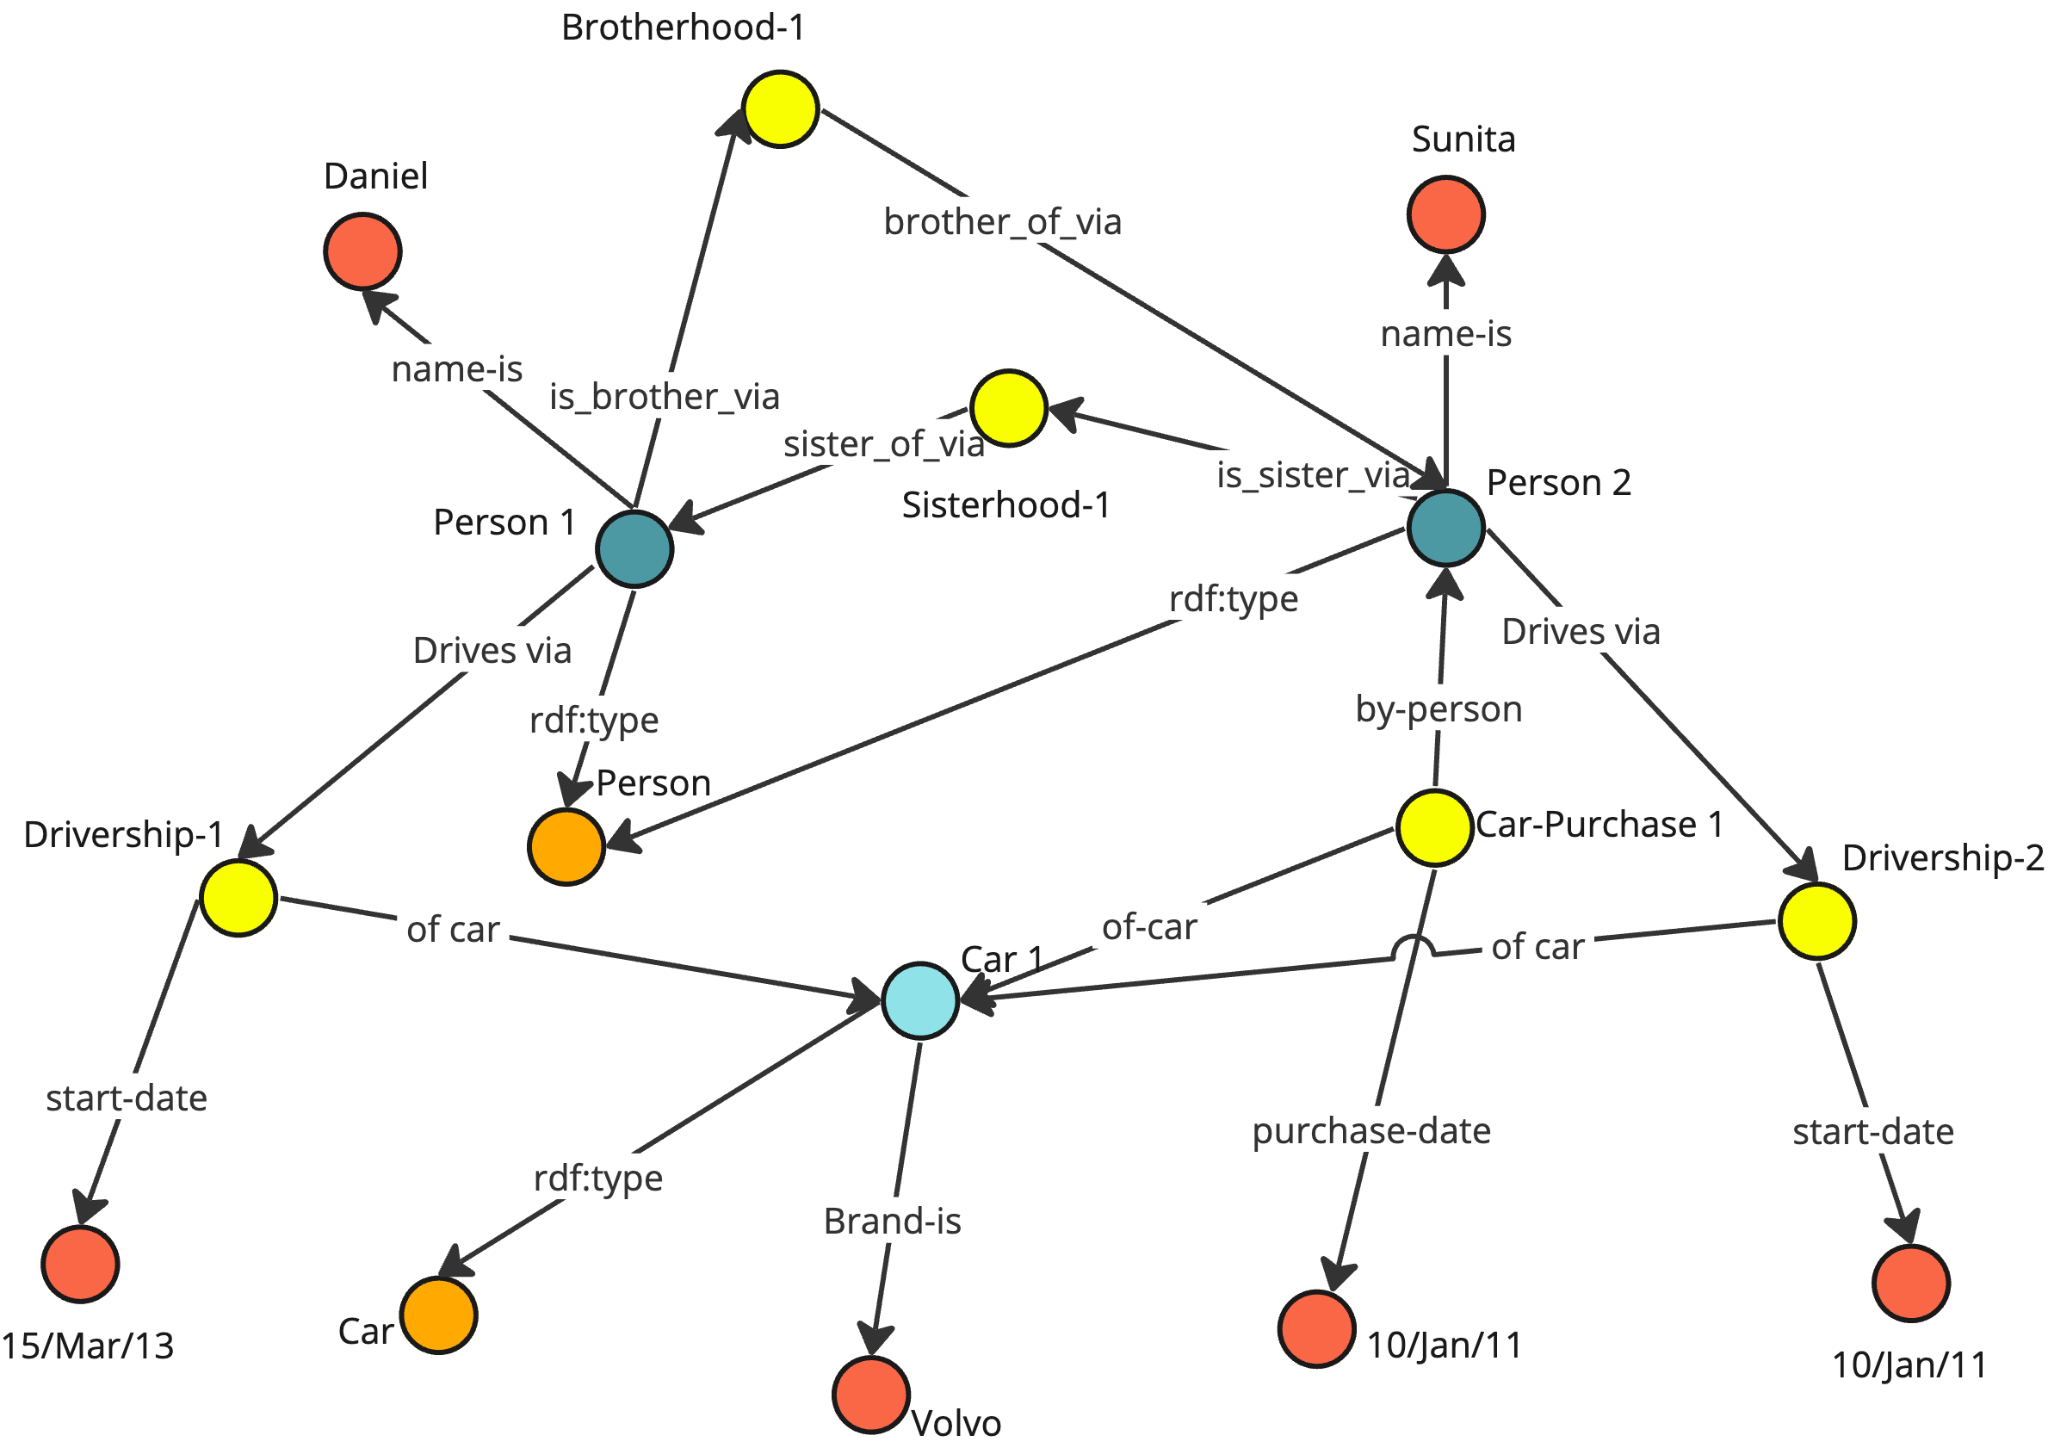
\includegraphics[width=0.82\textwidth]{image/static/rdf-model.png}
    \caption{Ví dụ mô hình RDF Graph, minh họa cách biểu diễn tri thức dưới dạng các bộ ba subject--predicate--object \cite{neo4j_rdf_vs_property}}
    \label{fig:rdf-graph}
\end{figure}

Như minh họa trong Hình \ref{fig:rdf-graph}, mỗi thông tin trong RDF thường được biểu diễn dưới dạng một bộ ba gồm subject, predicate và object. Mô hình này thuận lợi cho việc biểu diễn ngữ nghĩa và liên kết dữ liệu giữa các hệ thống khác nhau.

Bên cạnh RDF, Property Graph là một mô hình phổ biến trong các hệ quản trị cơ sở dữ liệu đồ thị hiện đại. Trong mô hình này, dữ liệu được biểu diễn bằng node và relationship; cả node và relationship đều có thể có nhãn và các thuộc tính dạng khóa--giá trị. Cách tổ chức này thuận tiện cho các bài toán cần truy vấn quan hệ, trực quan hóa graph và phát triển ứng dụng thực tế trên graph database \cite{angles2018property}.

\begin{figure}[H]
    \centering
    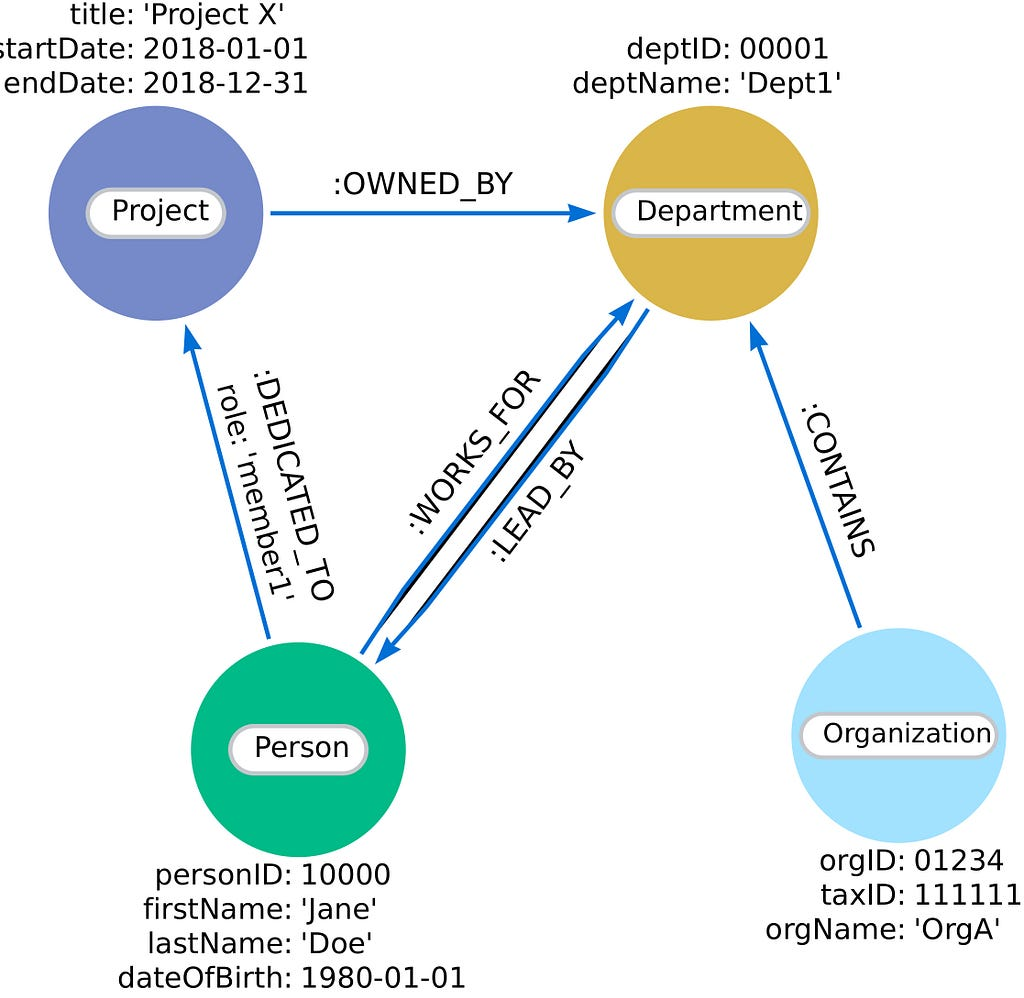
\includegraphics[width=0.78\textwidth]{image/static/property-graph.png}
    \caption{Ví dụ mô hình Property Graph, trong đó node và relationship có thể mang thuộc tính \cite{neo4j_property_graph_image}}
    \label{fig:property-graph}
\end{figure}

Hình \ref{fig:property-graph} cho thấy Property Graph cho phép lưu trữ trực tiếp thuộc tính trên cả node và relationship, từ đó giúp mô hình dữ liệu linh hoạt và gần với cách triển khai trong các graph database như Neo4j.

Trong khóa luận này, Knowledge Graph được triển khai theo hướng Property Graph vì dữ liệu đầu vào có tính bán cấu trúc, quan hệ trong dữ liệu đa dạng và hệ thống cần tích hợp với Neo4j để phục vụ lưu trữ, truy vấn và khai thác trong ứng dụng hỏi đáp. Ngoài ra, Property Graph cũng phù hợp với ngôn ngữ truy vấn Cypher, vốn được thiết kế để thao tác trực tiếp trên các mẫu node--relationship trong graph \cite{francis2018cypher}. Tuy nhiên, việc lựa chọn Property Graph không có nghĩa là bỏ qua vai trò của ontology. Ngược lại, khóa luận vẫn sử dụng schema định hướng để đảm bảo nhãn thực thể, kiểu quan hệ và thuộc tính có tính nhất quán trong quá trình trích xuất và lưu trữ tri thức.

\section{Ontology trong xây dựng Knowledge Graph}

Ontology là một mô hình mô tả các khái niệm, quan hệ và ràng buộc trong một miền tri thức \cite{gruber1993translation}. Trong quá trình xây dựng Knowledge Graph, ontology đóng vai trò như một khung định hướng, hay schema, giúp xác định những loại thực thể nào cần được biểu diễn, các quan hệ nào có thể xuất hiện và những thuộc tính nào cần được lưu trữ \cite{hogan2021knowledge}. Một quy trình phát triển ontology thường bắt đầu từ việc xác định miền và phạm vi, liệt kê các khái niệm quan trọng, tổ chức chúng thành lớp, xác định thuộc tính và ràng buộc của các lớp \cite{noy2001ontology}.

Đối với miền thông tin về Đại học Công nghệ, ontology có thể bao gồm các nhóm khái niệm như tổ chức, đơn vị trực thuộc, con người, chương trình đào tạo, sự kiện, văn bản, học bổng, thông báo và nền tảng số. Việc xác định trước các nhóm khái niệm và kiểu quan hệ này giúp định hướng quá trình trích xuất thông tin bằng LLM theo một schema nhất quán hơn. Nhờ đó, hệ thống có thể giảm tình trạng sinh ra các nhãn thực thể tùy tiện, quan hệ không thống nhất hoặc thông tin thiếu căn cứ trong quá trình trích xuất \cite{pan2024unifying}.

Trong khóa luận này, ontology không được xây dựng theo hướng một ontology hình thức đầy đủ với toàn bộ ràng buộc logic phức tạp. Thay vào đó, ontology được sử dụng như một schema định hướng cho quá trình trích xuất và lưu trữ dưới dạng Property Graph. Cách tiếp cận này phù hợp với mục tiêu thực tế của hệ thống: xây dựng một graph có thể khai thác được cho ứng dụng hỏi đáp, đồng thời vẫn duy trì mức độ nhất quán cần thiết về nhãn thực thể, kiểu quan hệ và thuộc tính \cite{angles2018property}.

\section{Trích xuất thông tin bằng mô hình ngôn ngữ lớn}

Information Extraction là bài toán trích xuất thông tin có cấu trúc từ dữ liệu phi cấu trúc hoặc bán cấu trúc. Trong các hệ thống truyền thống, bài toán này thường được giải quyết bằng rule-based extraction, mô hình học máy có giám sát hoặc các mô hình nhận dạng thực thể. Tuy nhiên, các phương pháp này thường đòi hỏi tập dữ liệu gán nhãn lớn hoặc các tập luật được xây dựng thủ công cho từng miền cụ thể, khiến quá trình thu nhận tri thức tốn nhiều chi phí khi chuyển sang miền dữ liệu mới \cite{ji2021survey}.

Sự phát triển của LLM mở ra khả năng trích xuất tri thức thông qua prompt engineering. Thay vì huấn luyện lại mô hình, hệ thống có thể mô tả nhiệm vụ, định nghĩa schema đầu ra và các ràng buộc trực tiếp trong prompt, sau đó yêu cầu LLM sinh kết quả theo định dạng mong muốn. Cách tiếp cận này đặc biệt phù hợp trong giai đoạn xây dựng nguyên mẫu hoặc với các miền tri thức mà dữ liệu gán nhãn còn hạn chế \cite{pan2024unifying}.

Tuy nhiên, prompt-based Information Extraction cũng đối mặt với nhiều thách thức. LLM có thể sinh sai định dạng, bỏ sót thực thể, tạo ra quan hệ không tồn tại trong văn bản gốc, hoặc sử dụng nhãn không nhất quán. Các lỗi này liên quan trực tiếp đến hiện tượng hallucination, tức mô hình sinh ra nội dung không được hỗ trợ đầy đủ bởi nguồn thông tin đầu vào \cite{ji2023survey}. Đối với tiếng Việt, bài toán càng phức tạp do đặc thù về tên riêng, tên tổ chức, từ ghép và sự đa dạng trong cách viết tắt \cite{nguyen2021phonlp}. Vì vậy, hệ thống cần kết hợp prompt có ràng buộc schema, bước kiểm tra đầu ra và cơ chế xử lý lỗi sau trích xuất.

Trong KGsAuto, LLM được sử dụng để đọc nội dung Markdown và sinh ra các graph fragment gồm danh sách node và relationship ở dạng JSON. Prompt được thiết kế để chỉ dẫn mô hình về nhóm thực thể, kiểu thông tin cần trích xuất, yêu cầu provenance và định dạng đầu ra. Bên cạnh đó, hệ thống sử dụng cơ chế sinh ID tất định dựa trên nội dung thực thể và quan hệ, giúp các artifact sau trích xuất ổn định hơn giữa các lần chạy. Các bước xử lý sau trích xuất tiếp tục phân biệt rõ thực thể đơn lẻ với các cụm thực thể được hợp nhất ở giai đoạn Entity Resolution. Đây là nền tảng cho quy trình xây dựng Knowledge Graph được trình bày chi tiết ở Chương 4.

\section{Entity Resolution trong Knowledge Graph}

Entity Resolution là bài toán phát hiện và hợp nhất các bản ghi hoặc thực thể khác nhau nhưng cùng biểu diễn một đối tượng trong thế giới thực \cite{christen2012data,papadakis2020entity}. Trong Knowledge Graph được trích xuất từ nhiều tài liệu, cùng một thực thể có thể xuất hiện dưới nhiều dạng tên khác nhau. Ví dụ, một tổ chức có thể được gọi bằng tên đầy đủ, tên viết tắt hoặc tên tiếng Anh; một cá nhân có thể xuất hiện cùng với học hàm, học vị hoặc chức vụ; một đơn vị có thể được nhắc đến trong nhiều bài viết với cách viết không hoàn toàn giống nhau.

Nếu không xử lý Entity Resolution, graph sau trích xuất sẽ chứa nhiều node trùng lặp. Điều này làm giảm chất lượng truy vấn, gây phân mảnh thông tin và ảnh hưởng trực tiếp đến chất lượng truy xuất cũng như câu trả lời của hệ thống hỏi đáp. Một câu hỏi về một đơn vị có thể chỉ truy xuất được một phần thông tin nếu các thông tin liên quan bị phân tán ở nhiều node khác nhau. Trong các hệ thống Knowledge Graph, canonicalization và curation là các bước quan trọng để duy trì chất lượng tri thức trong vòng đời của graph \cite{weikum2021machine}.

Các phương pháp Entity Resolution thường kết hợp nhiều kỹ thuật như chuẩn hóa chuỗi, so khớp fuzzy, embedding similarity, blocking, clustering và xác thực bằng mô hình học máy hoặc LLM \cite{papadakis2020entity}. Blocking giúp giảm không gian tìm kiếm các cặp cần so sánh; embedding giúp biểu diễn thực thể trong không gian vector; clustering nhóm các thực thể có khả năng trùng lặp. Các nghiên cứu gần đây cũng cho thấy LLM có tiềm năng hỗ trợ entity matching trong các trường hợp tên gọi phức tạp hoặc cần hiểu ngữ cảnh \cite{peeters2023using}.

Trong khóa luận này, Entity Resolution được xem là một bước độc lập sau trích xuất. Pipeline gồm ba giai đoạn: chuẩn hóa và tạo embedding, blocking và clustering, sau đó xác thực bằng LLM và tổng hợp canonical entity. Để tăng tính minh bạch, hệ thống phân biệt rõ các thực thể không qua hợp nhất với các cụm thực thể đã được hợp nhất. Cách báo cáo này giúp đánh giá chính xác tác động của Entity Resolution thay vì chỉ nhìn vào số lượng thực thể sau xử lý. Quy trình này được trình bày chi tiết trong Chương 5.

\section{Retrieval-Augmented Generation và Graph-based RAG}

Retrieval-Augmented Generation là kiến trúc kết hợp giữa truy xuất thông tin và sinh ngôn ngữ \cite{lewis2020retrieval}. Thay vì để LLM trả lời chỉ dựa trên tham số đã học, hệ thống RAG truy xuất các đoạn tài liệu liên quan đến câu hỏi, đưa các đoạn này vào prompt và yêu cầu LLM sinh câu trả lời dựa trên ngữ cảnh được cung cấp. Cách tiếp cận này giúp cải thiện tính cập nhật của tri thức và giảm nguy cơ sinh câu trả lời không có căn cứ.

RAG truyền thống thường dựa trên semantic search, trong đó tài liệu được chia thành các chunk, chuyển thành embedding và lưu trong vector database. Khi người dùng đặt câu hỏi, hệ thống tìm các chunk gần nhất trong không gian vector. Tuy nhiên, semantic search có hạn chế khi câu hỏi yêu cầu hiểu quan hệ có cấu trúc, truy vấn nhiều bước hoặc tổng hợp thông tin từ nhiều thực thể liên quan \cite{gao2023retrieval}.

Graph-based RAG bổ sung Knowledge Graph vào quá trình truy xuất để hỗ trợ các câu hỏi cần khai thác quan hệ có cấu trúc \cite{edge2024local}. Thay vì chỉ tìm đoạn văn bản gần nghĩa, hệ thống có thể truy xuất node, relationship và path trong graph. Điều này giúp biểu diễn rõ bằng chứng theo quan hệ và hỗ trợ các câu hỏi như “đơn vị nào trực thuộc tổ chức nào”, “ai giữ vai trò gì”, hoặc “sự kiện nào liên quan đến đơn vị nào”.

Trong khóa luận này, hệ thống sử dụng cả semantic search trên văn bản gốc và truy xuất trên Knowledge Graph. Cách kết hợp này cho phép tận dụng ưu điểm của hai nguồn bằng chứng: văn bản gốc cung cấp nội dung chi tiết, trong khi graph cung cấp cấu trúc quan hệ giữa các thực thể. Trên cơ sở đó, hệ thống hỏi đáp được thiết kế với nhiều chế độ truy xuất gồm Semantic Search, Graph Search, Naive Graph RAG và Hybrid RAG. Các chế độ này được trình bày trong Chương 6.

\section{Các công nghệ sử dụng}

Hệ thống KGsAuto sử dụng một số công nghệ chính phục vụ cho các tầng khác nhau của pipeline. Neo4j được sử dụng làm graph database để lưu trữ và truy vấn Knowledge Graph. Neo4j phù hợp với mô hình Property Graph và hỗ trợ truy vấn quan hệ bằng Cypher.

Qdrant được sử dụng làm vector database để lưu trữ embedding của các đoạn văn bản hoặc thực thể. Trong hệ thống, Qdrant phục vụ hai vai trò: hỗ trợ truy xuất markdown chunk trong RAG và hỗ trợ lưu trữ vector trong một số bước của Entity Resolution.

FastAPI được sử dụng để xây dựng backend API và RAG API. Backend cung cấp các chức năng tìm kiếm, truy vấn graph, xem chi tiết thực thể và merge thực thể. RAG API cung cấp giao diện truy vấn cho các chế độ hỏi đáp.

React/Vite được sử dụng để xây dựng frontend cho người dùng cuối. Giao diện hỗ trợ các luồng cơ bản như tìm kiếm, xem trang thực thể, quan sát quan hệ và thao tác merge trong trường hợp cần hiệu chỉnh graph.

Ngoài ra, hệ thống sử dụng Sentence Transformers để tạo embedding và một lớp trừu tượng LLM provider để gọi các mô hình ngôn ngữ khác nhau trong quá trình trích xuất, đối soát thực thể và sinh câu trả lời.

\clearpage

% Chapter 3: Quy trình trích xuất
\chapter{Kiến trúc tổng thể của quy trình xây dựng đồ thị tri thức}

Chương này trình bày bức tranh tổng thể của quy trình xây dựng đồ thị tri thức từ dữ liệu văn bản tiếng Việt phi cấu trúc. Mục tiêu của chương không phải là mô tả chi tiết từng kỹ thuật xử lý, mà là làm rõ các khối chức năng chính, vai trò của từng khối và cách chúng nối tiếp nhau trong toàn bộ quy trình. Các bước cụ thể của từng thành phần sẽ được trình bày ở các chương sau.

Trong phạm vi khóa luận, dữ liệu đầu vào là các tài liệu công khai về Trường Đại học Công nghệ, Đại học Quốc gia Hà Nội. Các tài liệu này chứa thông tin về đơn vị, cán bộ, chương trình đào tạo, thông báo, sự kiện, văn bản và các hoạt động liên quan đến nhà trường. Đặc điểm chung của nguồn dữ liệu là thông tin phân tán ở nhiều bài viết, cùng một đối tượng có thể xuất hiện dưới nhiều cách gọi khác nhau, và nhiều quan hệ giữa các đối tượng không được biểu diễn sẵn dưới dạng có cấu trúc. Vì vậy, quy trình xây dựng đồ thị tri thức cần giải quyết ba vấn đề chính: trích xuất tri thức từ văn bản, hợp nhất các thực thể trùng lặp và kiểm soát các trường hợp không đủ chắc chắn bằng sự can thiệp của con người (human fallback).

\begin{figure}[H]
    \centering
    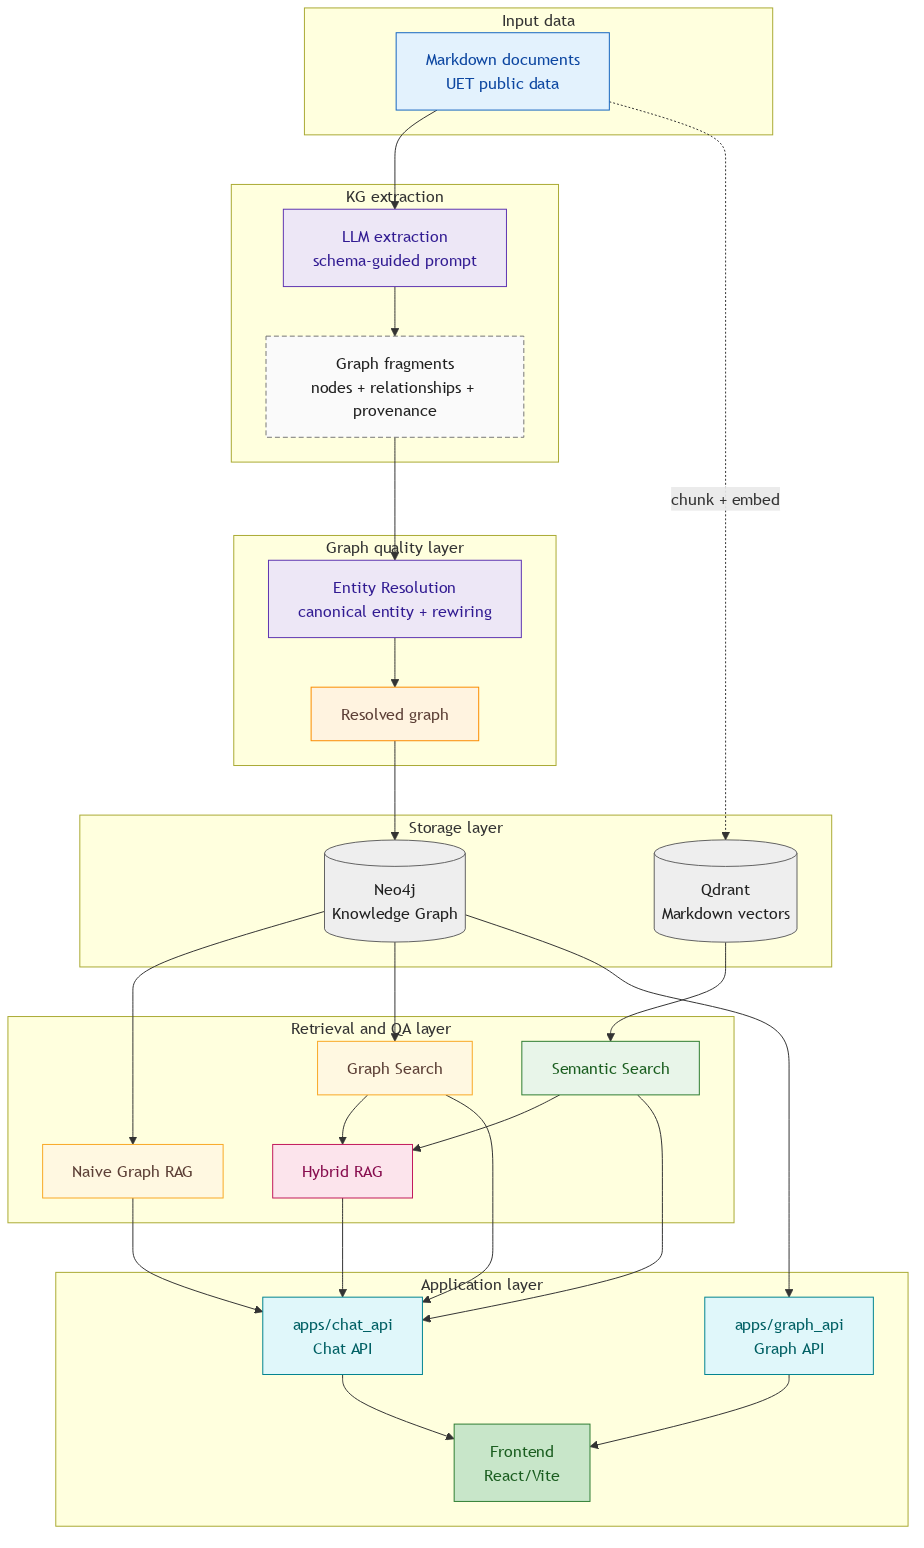
\includegraphics[width=\textwidth]{image/generated/chapter3/architecture-overview.png}
    \caption{Kiến trúc tổng thể của quy trình xây dựng đồ thị tri thức}
    \label{fig:architecture-overview}
\end{figure}

Hình~\ref{fig:architecture-overview} mô tả quy trình ở mức tổng quan thông qua năm khối chính. Khối dữ liệu tiếp nhận các tài liệu văn bản đã được xử lý và gắn thông tin nguồn. Từ dữ liệu này, hệ thống thực hiện trích xuất tri thức để nhận diện thực thể, quan hệ và bằng chứng văn bản tương ứng. Kết quả sau trích xuất vẫn là các mảnh tri thức ban đầu, nên cần được đưa sang bước xử lý đồng tham chiếu để phát hiện các biến thể tên gọi và hợp nhất các thực thể cùng tham chiếu đến một đối tượng.

Sau bước xử lý đồng tham chiếu, các trường hợp mơ hồ hoặc có rủi ro hợp nhất sai được chuyển sang human fallback để con người kiểm chứng trước khi chấp nhận quyết định cuối cùng. Kết quả của toàn bộ quy trình là một đồ thị tri thức có cấu trúc, trong đó thực thể và quan hệ được tổ chức nhất quán hơn và vẫn có thể truy vết về nguồn văn bản ban đầu thông qua \texttt{chunk\_id}, metadata và bằng chứng đi kèm. Các chi tiết kỹ thuật của từng khối, như gom nhóm chunks, thiết kế prompt, chuẩn hóa thực thể, embedding và tìm kiếm ứng viên đồng tham chiếu, được trình bày ở các chương tiếp theo.

\begin{figure}[H]
    \centering
    \makebox[\textwidth][c]{%
        \begin{minipage}[t]{0.54\textwidth}
            \centering
            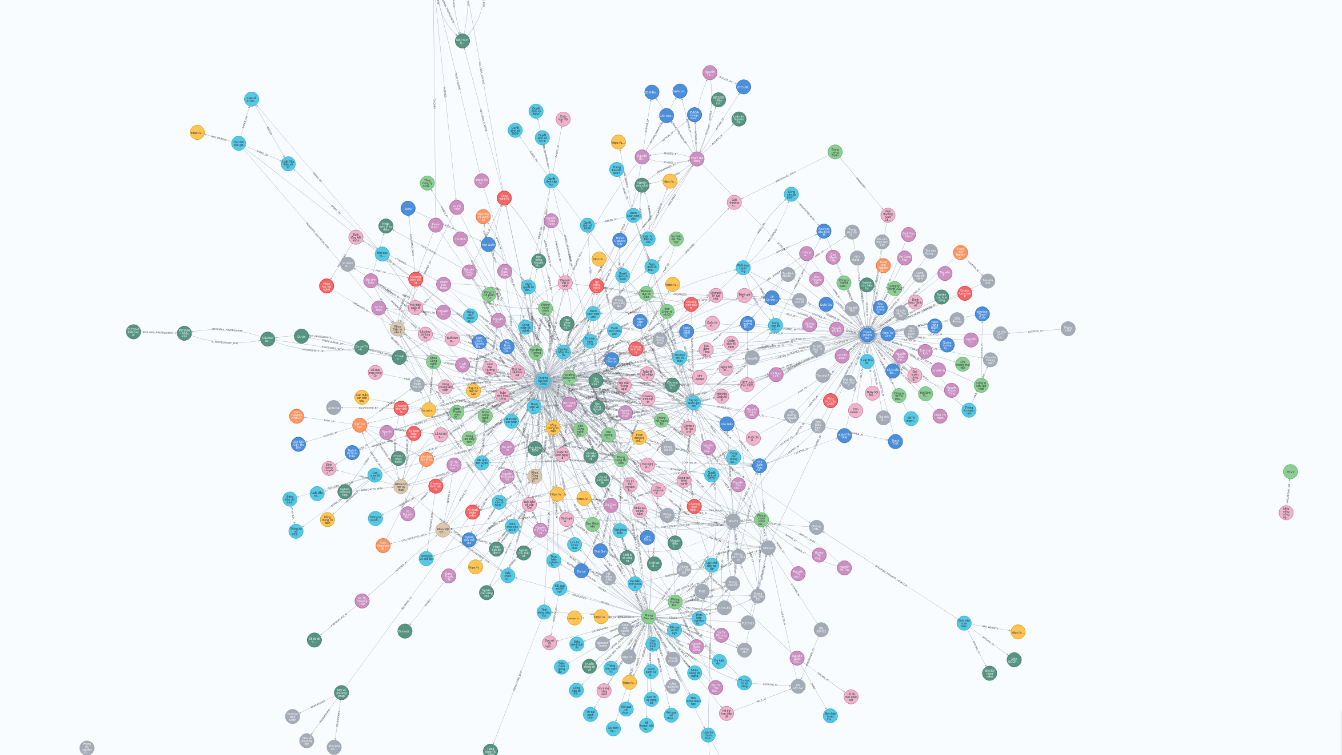
\includegraphics[width=\linewidth]{image/static/raw_graph_visualize.png}
            \vspace{2pt}
            {\small (a) Đồ thị thô sau trích xuất}
        \end{minipage}%
        \hspace{0.02\textwidth}%
        \begin{minipage}[t]{0.54\textwidth}
            \centering
            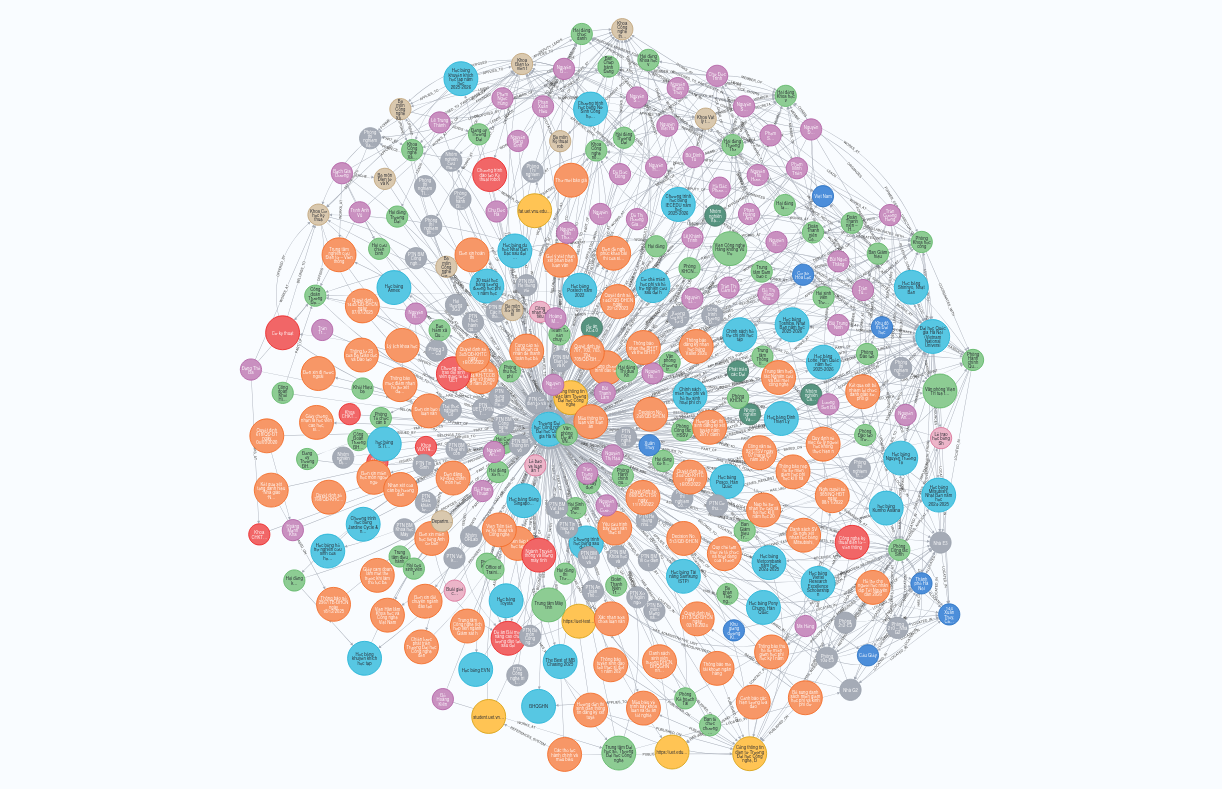
\includegraphics[width=\linewidth]{image/static/graph_visualize.png}
            \vspace{2pt}
            {\small (b) Đồ thị sau tổ chức và hợp nhất}
        \end{minipage}%
    }
    \vspace{6pt}

    \makebox[\textwidth][c]{%
        \begin{minipage}[t]{1.08\textwidth}
            \centering
            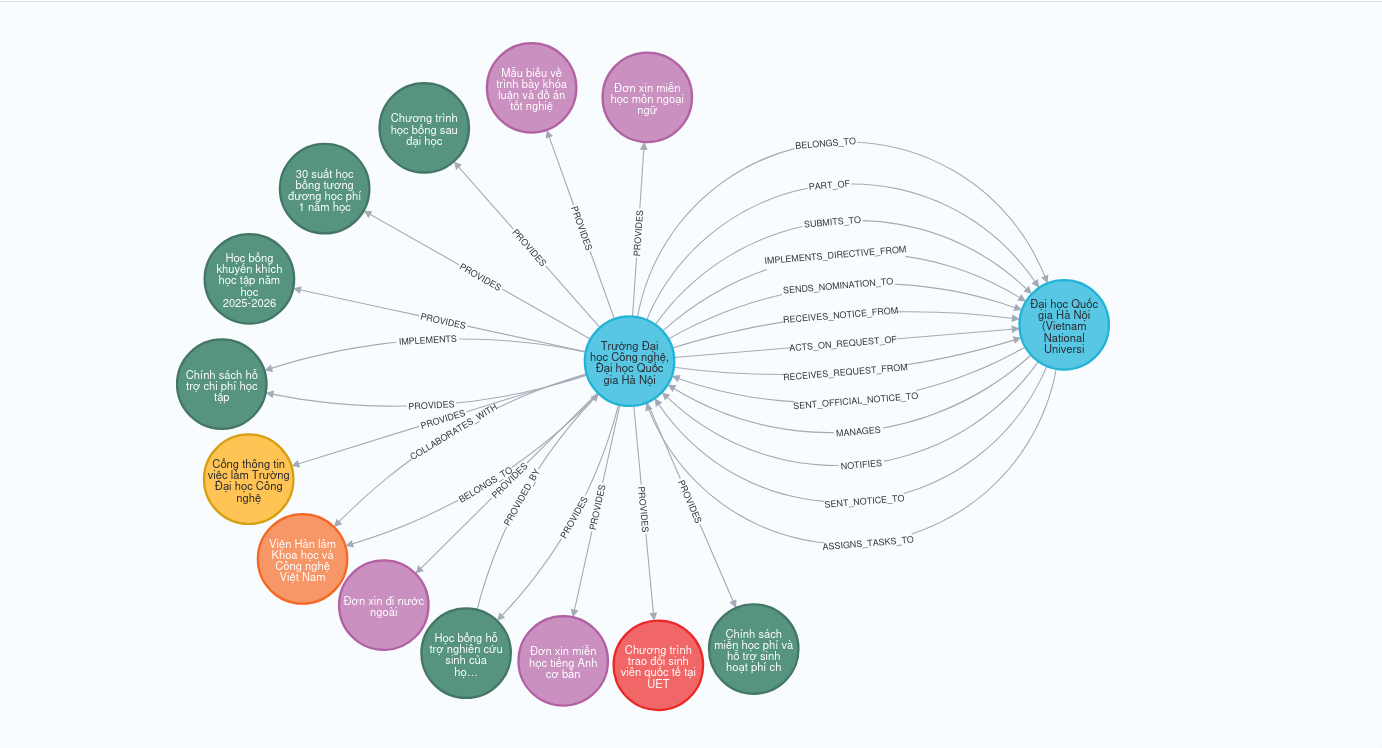
\includegraphics[width=\linewidth]{image/static/mini_graph_visualize.png}
            \vspace{2pt}
            {\small (c) Minh họa với 15 thực thể}
        \end{minipage}%
    }
    \caption{So sánh đồ thị tri thức trước và sau khi tổ chức các thực thể và quan hệ}
    \label{fig:graph-visualize}
\end{figure}

Hình~\ref{fig:graph-visualize} minh họa sự thay đổi của đồ thị tri thức trong quy trình xử lý. Ở bên trái, đồ thị thô sau trích xuất còn phân tán và chứa nhiều cụm rời rạc do các thực thể được tạo từ từng tài liệu hoặc từng phân đoạn riêng lẻ. Ở bên phải, sau khi tổ chức lại thực thể, hợp nhất các trường hợp đồng tham chiếu và cập nhật quan hệ, đồ thị trở nên tập trung hơn, giúp quan sát rõ hơn các liên kết giữa các đối tượng và tạo nền tảng tốt hơn cho phần đánh giá hỏi đáp ở Chương~6.

Từ kiến trúc tổng thể này, các chương tiếp theo đi vào từng phần của quy trình. Chương 4 trình bày quy trình trích xuất tri thức từ dữ liệu. Chương 5 trình bày xử lý đồng tham chiếu thực thể và cơ chế human fallback. Chương 6 trình bày thực nghiệm và đánh giá, trong đó phần hỏi đáp được dùng để kiểm tra giá trị sử dụng của đồ thị tri thức ở lớp ứng dụng.

\clearpage

% Chapter 4: Xây dựng câu lệnh (Prompt)
\chapter{Trích xuất tri thức từ dữ liệu}

\section{Tổng quan quy trình trích xuất}

Mục tiêu của quy trình trích xuất là chuyển đổi dữ liệu phi cấu trúc thành các mảnh tri thức ban đầu có thể tổ chức trong đồ thị. Ở giai đoạn này, hệ thống chưa tạo ra đồ thị tri thức cuối cùng, mà tập trung nhận diện các đối tượng quan trọng, các quan hệ có căn cứ trong tài liệu và thông tin nguồn để phục vụ kiểm tra ở các bước sau.

Ở mức tổng quan, quy trình trích xuất gồm bốn nhóm chức năng chính. Nhóm thứ nhất chuẩn bị và tổ chức dữ liệu đầu vào để nội dung được xử lý theo các đơn vị rõ ràng. Nhóm thứ hai xác định ngữ cảnh và các quy tắc biểu diễn tri thức, giúp kết quả trích xuất thống nhất hơn giữa nhiều tài liệu. Nhóm thứ ba nhận diện thực thể, thuộc tính và quan hệ xuất hiện trong văn bản. Nhóm thứ tư kiểm tra, làm sạch và lưu lại kết quả cùng thông tin truy vết nguồn gốc.

Đầu ra của quy trình trích xuất là một đồ thị thô, đóng vai trò dữ liệu trung gian cho toàn bộ quy trình xây dựng đồ thị tri thức. Đồ thị thô này vẫn có thể chứa thực thể trùng lặp, đồng tham chiếu, quan hệ chưa nhất quán hoặc thông tin cần được kiểm tra thêm. Vì vậy, kết quả sau trích xuất sẽ được chuyển sang bước xử lý đồng tham chiếu thực thể ở Chương~5 để giảm phân mảnh và nâng cao tính nhất quán của đồ thị. Quy trình tổng quan được minh họa trong Hình~\ref{fig:extraction-pipeline}.

\begin{figure}[H]
    \centering
    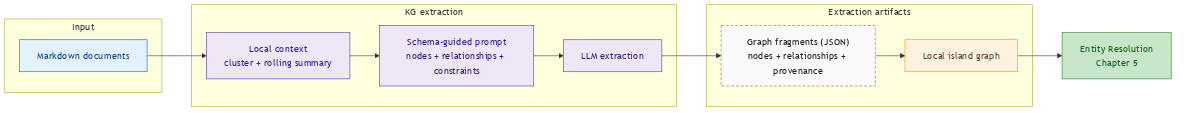
\includegraphics[width=\textwidth]{image/generated/chapter4/extraction-pipeline.png}
    \caption{Quy trình trích xuất tri thức từ dữ liệu}
    \label{fig:extraction-pipeline}
\end{figure}

\section{Xử lý và phân đoạn dữ liệu}

Dữ liệu đầu vào của khóa luận được thu thập tự động từ các trang tin tức công khai của Trường Đại học Công nghệ. Dữ liệu sau khi thu thập thường chưa ở trạng thái phù hợp để trích xuất tri thức trực tiếp, vì nội dung trên trang tin tức có thể chứa nhiều thành phần không cần thiết như thanh điều hướng, chân trang, liên kết lặp lại hoặc các đoạn văn bản không mang nhiều thông tin. Do đó, bước xử lý dữ liệu có nhiệm vụ làm sạch nội dung và đưa dữ liệu về một dạng biểu diễn thống nhất.

Trong khóa luận này, dữ liệu sau khi xử lý được chuẩn hóa về dạng Markdown. Dạng biểu diễn này giữ lại được cấu trúc cơ bản của tài liệu như tiêu đề, đoạn văn, danh sách và liên kết, đồng thời loại bỏ bớt các yếu tố trình bày không cần thiết của trang tin tức. Việc chuẩn hóa dữ liệu giúp các bước sau làm việc với một đầu vào nhất quán hơn, thay vì phải xử lý trực tiếp nhiều dạng nội dung khác nhau từ các trang tin tức.

Một vấn đề quan trọng trong giai đoạn này là lượng dữ liệu đầu vào ảnh hưởng trực tiếp đến chất lượng kết quả trích xuất. Mô hình ngôn ngữ lớn chỉ có thể xử lý một lượng ngữ cảnh hữu hạn trong mỗi lần suy luận. Nếu đưa một tài liệu quá dài hoặc quá nhiều tài liệu vào cùng một lần xử lý, nội dung có thể vượt quá giới hạn ngữ cảnh của mô hình, làm mất thông tin quan trọng hoặc khiến kết quả đầu ra thiếu ổn định. Ngược lại, nếu chia dữ liệu quá nhỏ, các đoạn văn bản có thể mất ngữ cảnh cần thiết để nhận diện đúng thực thể và quan hệ.

Vì vậy, dữ liệu cần được phân đoạn trước khi đưa vào bước trích xuất tri thức. Phân đoạn dữ liệu, hay chunking, là quá trình chia nội dung thành các đơn vị xử lý nhỏ hơn nhưng vẫn cố gắng giữ được ý nghĩa tương đối đầy đủ của từng đoạn. Cách tổ chức này giúp hạn chế tình trạng tràn ngữ cảnh của mô hình ngôn ngữ lớn, đồng thời tạo điều kiện để hệ thống kiểm soát tốt hơn chất lượng đầu vào cho từng lần trích xuất.

Trong quá trình xử lý, mỗi tài liệu hoặc phân đoạn dữ liệu được gắn với thông tin nguồn tương ứng. Thông tin này cho phép truy ngược kết quả trích xuất về tài liệu ban đầu, hỗ trợ kiểm tra bằng chứng và sửa lỗi khi cần thiết. Như vậy, bước xử lý và phân đoạn dữ liệu không chỉ chuẩn bị đầu vào cho mô hình, mà còn đặt nền tảng cho tính minh bạch và khả năng kiểm chứng của đồ thị tri thức ở các bước sau.

\section{Gom nhóm dữ liệu và duy trì ngữ cảnh}

Sau khi dữ liệu được xử lý và phân đoạn, mỗi đoạn dữ liệu (chunk) vẫn chỉ chứa một phần ngữ cảnh của toàn bộ nguồn dữ liệu. Một chủ đề có thể được phân tán trên nhiều trang khác nhau, trong khi cùng một thực thể có thể xuất hiện dưới nhiều cách gọi như tên đầy đủ, tên viết tắt hoặc tên theo ngữ cảnh. Nếu từng đoạn dữ liệu được đưa vào trích xuất một cách hoàn toàn độc lập, các phiên trích xuất dễ tạo ra những mảnh tri thức rời rạc, thiếu liên kết với nhau. Vì vậy, bước gom nhóm dữ liệu được sử dụng để đưa các đoạn có khả năng liên quan vào cùng một nhóm, dựa trên nguyên tắc tương đồng nội dung (content similarity).

Mục tiêu của việc gom nhóm trong giai đoạn này không phải là giải quyết triệt để bài toán đồng tham chiếu thực thể. Việc hợp nhất thực thể ở phạm vi toàn cục sẽ được trình bày ở Chương~5. Ở đây, bước gom nhóm đóng vai trò giảm bớt sự rời rạc ban đầu của dữ liệu, giúp các đoạn cùng chủ đề hoặc cùng nhắc đến một nhóm thực thể được xử lý gần nhau hơn. Có thể xem kết quả của bước này là các nhóm đoạn liên quan (related chunks), tạo điều kiện để hệ thống tái sử dụng thông tin đã trích xuất trước đó trong phạm vi nhóm, thay vì xử lý từng đoạn như những đơn vị hoàn toàn tách biệt.

Cách thực hiện gom nhóm bắt đầu từ việc biểu diễn mỗi đoạn bằng một tập từ khóa đại diện. Trong cài đặt của khóa luận, các từ khóa này được lấy từ tên tệp hoặc đường dẫn sau khi đã chuẩn hóa, sau đó loại bỏ những từ ít mang ý nghĩa. Hệ thống tính độ tương đồng Jaccard giữa các tập từ khóa để ước lượng mức độ gần nhau giữa hai đoạn. Nếu độ tương đồng vượt qua một ngưỡng định trước, các đoạn được đưa vào cùng một nhóm; nếu không, hệ thống tạo nhóm mới. Đây là một cách cài đặt cụ thể của nguyên tắc gom nhóm theo tương đồng nội dung, phù hợp với dữ liệu thu thập từ trang tin tức vì tên trang và đường dẫn thường phản ánh chủ đề chính của nội dung.

Sau khi có các nhóm dữ liệu, hệ thống cần duy trì ngữ cảnh cục bộ (local context) bên trong từng nhóm. Với mỗi nhóm, local context ban đầu rỗng. Sau khi một đoạn được trích xuất thành công, hệ thống lưu lại các thực thể quan trọng, tên gọi thay thế và một số quan hệ hoặc sự kiện vừa nhận diện được. Phần ngữ cảnh này được cập nhật dần theo kiểu tóm tắt cuốn chiếu (rolling summary), rồi được đưa vào đầu vào của mô hình khi xử lý đoạn tiếp theo trong cùng nhóm. Nhờ đó, mô hình có thêm căn cứ để nhận diện lại các thực thể đã xuất hiện trước đó và giảm sự thiếu nhất quán giữa các lần trích xuất.

Nhờ local context, các phiên trích xuất trong cùng một nhóm không còn hoàn toàn độc lập. Ví dụ, nếu một đoạn trước đã ghi nhận Trường Đại học Công nghệ, Đại học Công nghệ và UET là các cách gọi liên quan đến cùng một đơn vị, đoạn sau trong cùng nhóm có thêm tín hiệu để sử dụng tên gọi nhất quán hơn. Cơ chế này giúp giảm một phần sự phân mảnh ngay từ giai đoạn trích xuất, đồng thời tạo đầu vào tốt hơn cho bước xử lý đồng tham chiếu thực thể ở chương tiếp theo.

\section{Xây dựng prompt trích xuất tri thức}

Prompt là phần chỉ dẫn đầu vào được gửi cho mô hình ngôn ngữ lớn để mô tả nhiệm vụ, cung cấp ngữ cảnh, đặt ra ràng buộc và quy định dạng kết quả cần sinh. Trong bài toán trích xuất tri thức, prompt không chỉ nêu yêu cầu mô hình đọc văn bản, mà còn chỉ rõ mô hình cần nhận diện loại thực thể nào, quan hệ nào được phép tạo, thông tin bằng chứng nào cần giữ lại và kết quả phải được biểu diễn theo cấu trúc nào.

Trong trích xuất tri thức bằng mô hình ngôn ngữ lớn, prompt có ảnh hưởng trực tiếp đến chất lượng và hình dạng của đồ thị được sinh ra. Cùng một đoạn văn bản có thể tạo ra các kết quả khác nhau nếu mô hình không được hướng dẫn rõ về phạm vi miền tri thức, kiểu thực thể cần nhận diện, kiểu quan hệ cần ưu tiên và cấu trúc đầu ra mong muốn. Vì vậy, prompt trong khóa luận không chỉ là một câu lệnh yêu cầu trích xuất thông tin, mà là cơ chế chuyển ontology và schema thành các chỉ dẫn cụ thể để kiểm soát quá trình sinh tri thức.

Ontology và schema là hai thành phần nền tảng trong quá trình xây dựng prompt. Ontology giúp xác định các khái niệm thuộc miền dữ liệu cần quan tâm, chẳng hạn trường đại học, đơn vị trực thuộc, chương trình đào tạo, cán bộ, sự kiện, văn bản hoặc địa điểm. Schema quy định cách các khái niệm đó được biểu diễn trong đồ thị, bao gồm kiểu thực thể, kiểu quan hệ, thuộc tính cần lưu và yêu cầu về bằng chứng. Theo Noy và McGuinness, xây dựng ontology cần bắt đầu từ việc xác định miền và phạm vi, liệt kê thuật ngữ quan trọng, xác định lớp, thuộc tính và các ràng buộc liên quan \cite{noy2001ontology}. Các nguyên tắc này được sử dụng trong khóa luận để xác định những loại tri thức cần trích xuất từ dữ liệu của Trường Đại học Công nghệ.

Qua quá trình nghiên cứu và thực nghiệm, có thể khái quát hai dạng cấu trúc prompt chính cho bài toán trích xuất tri thức. Dạng thứ nhất là prompt không kiểm soát kiểu thực thể và quan hệ, tức mô hình được để tự do quyết định đối tượng nào nên trở thành thực thể và quan hệ nào nên được sinh ra. Cách này có ưu điểm là linh hoạt, nhưng dễ tạo ra nhiều nhãn thực thể khác nhau cho cùng một loại đối tượng, nhiều tên quan hệ có nghĩa gần nhau nhưng cách viết khác nhau, và các mảnh đồ thị khó hợp nhất ở các bước sau.

Dạng thứ hai là prompt có kiểm soát, trong đó kiểu thực thể, định hướng quan hệ và quy tắc biểu diễn được xác định trước dựa trên ontology và schema. Cách này giúp đầu ra của mô hình ổn định hơn, dễ kiểm tra hơn và phù hợp hơn với mục tiêu xây dựng đồ thị tri thức có cấu trúc. Các nghiên cứu gần đây về xây dựng đồ thị tri thức bằng mô hình ngôn ngữ lớn cũng nhấn mạnh rằng trích xuất cần đi kèm với bước định nghĩa và chuẩn hóa tri thức, thay vì để mô hình sinh kết quả hoàn toàn tự do \cite{zhang2024extract}. Vì vậy, khóa luận lựa chọn hướng prompt có kiểm soát.

Cụ thể, khóa luận kiểm soát chặt các kiểu thực thể được phép tạo ra bằng một tập nhãn thực thể định nghĩa trước. Mô hình chỉ được tạo thực thể thuộc các kiểu nằm trong tập này, nhờ đó hạn chế tình trạng sinh nhãn tùy ý hoặc tạo nút cho các khái niệm quá chung. Đối với quan hệ, khóa luận sử dụng cách kiểm soát mềm hơn: prompt đưa ra các tên quan hệ được ưu tiên và các quy tắc sinh quan hệ để định hướng mô hình. Cách thiết kế này giữ được khả năng biểu diễn các quan hệ đa dạng trong văn bản tự nhiên, nhưng vẫn hạn chế các quan hệ dài, mơ hồ hoặc khó tái sử dụng. Trong những hệ thống yêu cầu quản lý chặt chẽ hơn, tập quan hệ cũng có thể được định nghĩa đóng hoàn toàn tương tự như tập kiểu thực thể.

Cấu trúc tổng thể của prompt trích xuất tri thức trong khóa luận gồm các phần chính sau. Phần mở đầu là hướng dẫn nhiệm vụ, nêu vai trò của mô hình và yêu cầu trích xuất thực thể, thuộc tính, quan hệ từ văn bản dựa trên bằng chứng. \texttt{ENTITY LABELS} định nghĩa tập kiểu thực thể được phép tạo ra; phần này thể hiện trực tiếp ảnh hưởng của ontology đối với phạm vi tri thức được trích xuất. \texttt{ENTITY RULES} quy định cách tạo thực thể, cách chọn tên chuẩn, cách xử lý tên viết tắt hoặc tên thay thế, và khi nào không nên tạo một thực thể mới. \texttt{PREFERRED RELATIONSHIP NAMES} cung cấp các tên quan hệ nên được ưu tiên tái sử dụng khi văn bản có liên kết phù hợp. \texttt{RELATIONSHIP RULES} quy định khi nào được tạo quan hệ, cách đặt tên quan hệ, yêu cầu quan hệ phải có căn cứ trong văn bản và cách mô tả liên kết giữa hai thực thể. \texttt{OUTPUT SCHEMA} định nghĩa cấu trúc đầu ra để kết quả có thể được kiểm tra, lưu trữ và chuyển sang các bước xử lý sau. Cuối cùng là phần văn bản đầu vào, tức đoạn dữ liệu đã được xử lý và đưa vào prompt để mô hình thực hiện trích xuất.

Hình~\ref{fig:kg-prompt} minh họa cấu trúc tổng thể của prompt trích xuất tri thức. Hình này cho thấy prompt được xây dựng từ nhiều lớp: hướng dẫn nhiệm vụ, ontology, schema, quy tắc thực thể, quy tắc quan hệ, cấu trúc đầu ra và văn bản đầu vào. Sự kết hợp này giúp quá trình trích xuất không chỉ dựa vào khả năng sinh ngôn ngữ của mô hình, mà còn được định hướng bởi các quyết định thiết kế tri thức của khóa luận.

\begin{figure}[H]
    \centering
    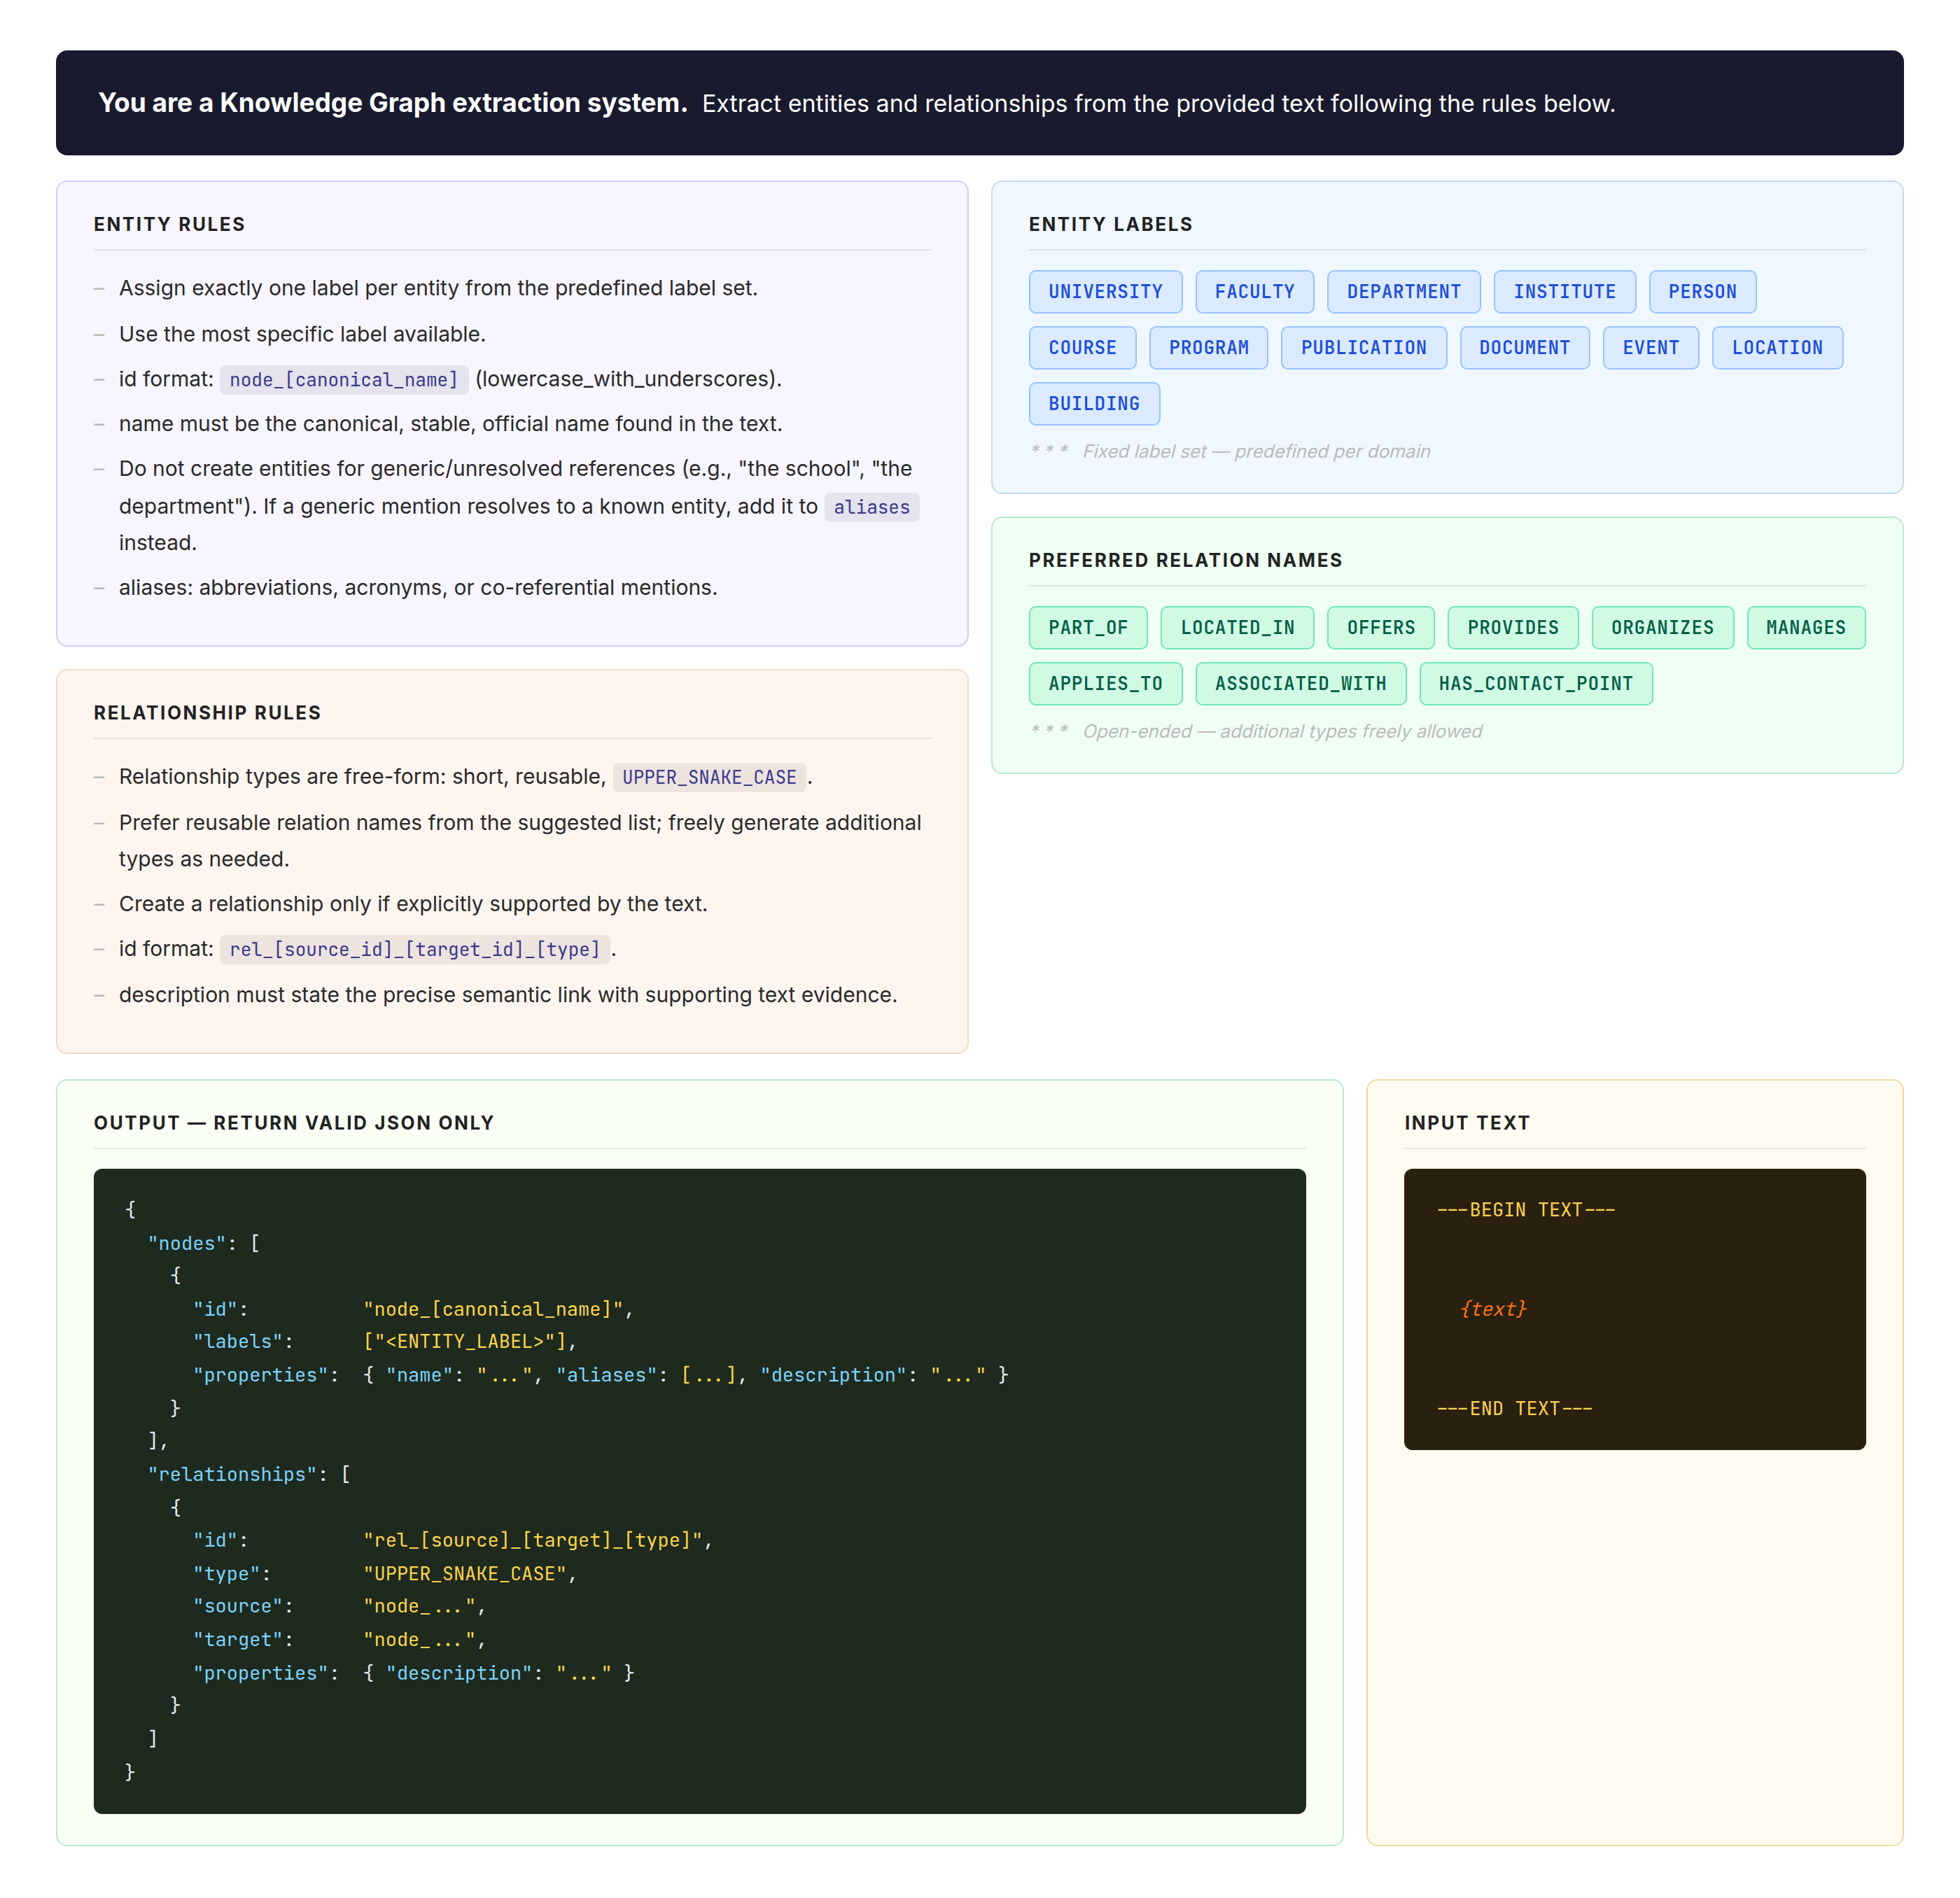
\includegraphics[width=\textwidth]{image/generated/chapter4/kg_prompt.png}
    \caption{Cấu trúc prompt trích xuất tri thức}
    \label{fig:kg-prompt}
\end{figure}

\section{Kết quả của trích xuất tri thức}

Sau khi áp dụng quy trình trích xuất trên tập dữ liệu đã thu thập, kết quả đầu ra là các mảnh đồ thị tri thức ở dạng JSON. Trong lần chạy hiện tại, quy trình xử lý 1.003 đơn vị dữ liệu và sinh ra 12.081 thực thể thô cùng 12.321 quan hệ thô. Các con số này phản ánh kết quả ngay sau giai đoạn trích xuất, trước khi thực hiện xử lý đồng tham chiếu thực thể và chuẩn hóa đồ thị ở Chương~5.

Kết quả sau trích xuất chưa phải là một đồ thị tri thức hoàn chỉnh. Do mỗi đoạn dữ liệu chỉ chứa một phần ngữ cảnh, đầu ra thường có dạng các đồ thị nhỏ rời rạc, mỗi đồ thị gắn với một tài liệu hoặc một phân đoạn cụ thể. Bên cạnh đó, cùng một đối tượng trong thực tế có thể được tạo thành nhiều thực thể khác nhau do khác biệt về tên đầy đủ, tên viết tắt, tên tiếng Anh hoặc cách gọi theo ngữ cảnh. Ví dụ, Trường Đại học Công nghệ có thể xuất hiện dưới các cách gọi như Trường ĐHCN, Đại học Công nghệ hoặc UET. Đặc điểm này cho thấy bước xử lý đồng tham chiếu thực thể là cần thiết để nối các mảnh đồ thị nhỏ thành một nguồn tri thức nhất quán hơn.

Ví dụ JSON - kết quả trích xuất. Trong ví dụ này, phần \texttt{nodes} chứa các thực thể được nhận diện từ văn bản, còn phần \texttt{relationships} chứa quan hệ giữa các thực thể đó. Các thuộc tính như \texttt{chunk\_id} và \texttt{description} giúp giữ lại liên kết với đoạn dữ liệu nguồn và bằng chứng mô tả.

\begin{jsonbox}
\{
  "nodes": [
    \{
      "id": "node\_uet",
      "labels": ["UNIVERSITY"],
      "properties": \{
        "name": "Đại học Công nghệ",
        "aliases": ["UET"],
        "chunk\_id": ["c1"],
        "description": ["Trường thành viên của ĐHQGHN."]
      \}
    \},
    \{
      "id": "node\_vnu",
      "labels": ["SYSTEM"],
      "properties": \{
        "name": "Đại học Quốc gia Hà Nội",
        "aliases": ["VNU"],
        "chunk\_id": ["c1"],
        "description": ["Trung tâm đại học lớn tại Việt Nam."]
      \}
    \}
  ],
  "relationships": [
    \{
      "id": "rel\_uet\_vnu\_MEMBER\_OF",
      "type": "MEMBER\_OF",
      "source": "node\_uet",
      "target": "node\_vnu",
      "properties": \{
        "chunk\_id": ["c1"],
        "description": ["UET trực thuộc VNU."]
      \}
    \}
  ]
\}
\end{jsonbox}

Đối với một thực thể trong \texttt{nodes}, trường \texttt{id} là định danh cục bộ của thực thể trong kết quả trích xuất. Trường \texttt{labels} cho biết kiểu thực thể, chẳng hạn trường đại học hoặc cá nhân. Phần \texttt{properties} lưu các thông tin mô tả của thực thể. Trong đó, \texttt{name} là tên chuẩn được chọn cho thực thể, \texttt{aliases} lưu các tên gọi thay thế hoặc tên viết tắt, \texttt{chunk\_id} cho biết đoạn dữ liệu nguồn, và \texttt{description} mô tả ngắn gọn bằng chứng hoặc thông tin chính được trích xuất từ văn bản.

Đối với một quan hệ trong \texttt{relationships}, trường \texttt{id} là định danh của quan hệ, trường \texttt{type} biểu diễn kiểu quan hệ, còn \texttt{source} và \texttt{target} lần lượt chỉ định hai thực thể ở hai đầu quan hệ. Các trường trong \texttt{properties} của quan hệ có vai trò tương tự như ở thực thể: lưu đoạn dữ liệu nguồn và phần mô tả giải thích vì sao quan hệ đó được tạo ra. Nhờ các trường này, mỗi thực thể và quan hệ trong đồ thị thô đều có thể được truy vết về nguồn dữ liệu ban đầu, hỗ trợ kiểm chứng, đánh giá chất lượng và sửa lỗi ở các bước sau.

Mặc dù prompt đã được kiểm soát bằng ontology và schema, trích xuất trực tiếp bằng mô hình ngôn ngữ lớn vẫn không thể tạo ngay một đồ thị tri thức hoàn chỉnh. Mô hình có thể bỏ sót thực thể hoặc quan hệ quan trọng khi thông tin được diễn đạt gián tiếp, có thể sinh quan hệ chưa đủ căn cứ nếu văn bản mơ hồ, hoặc tạo ra nhiều nút khác nhau cho cùng một đối tượng trong thực tế. Các nghiên cứu về tạo đồ thị tri thức bằng mô hình ngôn ngữ lớn cũng chỉ ra rằng sai lệch và suy diễn quá mức vẫn là rủi ro cần được kiểm soát khi mở rộng quy trình sinh tri thức \cite{parovic2025generating}.

Đối với dữ liệu tiếng Việt của Trường Đại học Công nghệ, vấn đề này càng rõ hơn do sự đa dạng của tên riêng, tên viết tắt và cách gọi không chính thức. Một đơn vị có thể được nhắc đến bằng tên đầy đủ, tên rút gọn, tên tiếng Anh hoặc chỉ bằng chức năng trong từng ngữ cảnh cụ thể. Nếu các biến thể này không được hợp nhất, đồ thị tri thức sẽ bị phân mảnh: quan hệ liên quan đến cùng một đối tượng bị chia ra nhiều nút, làm giảm khả năng truy vấn, tổng hợp và trả lời câu hỏi. Ngược lại, nếu hợp nhất sai các thực thể khác nhau, đồ thị có thể chứa các quan hệ không đúng.

Vì vậy, Chương~5 giữ vai trò then chốt trong toàn bộ quy trình xây dựng đồ thị tri thức. Chương này không chỉ là bước xử lý bổ sung sau trích xuất, mà là bước chuyển từ tập mảnh đồ thị thô sang một đồ thị tri thức có chất lượng tốt hơn. Thông qua việc phát hiện các thực thể đồng tham chiếu, chọn thực thể chuẩn, hợp nhất tên gọi thay thế và cập nhật lại các quan hệ, quy trình xử lý đồng tham chiếu thực thể giúp giảm phân mảnh, tăng tính nhất quán và tạo nền tảng đáng tin cậy hơn cho ứng dụng hỏi đáp ở các chương sau.

\clearpage

% Chapter 5: Đối soát thực thể
\chapter{Đồng tham chiếu thực thể trong Knowledge Graph}

\section{Phát biểu bài toán Entity Resolution}

Sau bước trích xuất tri thức (Chương 4), đồ thị đầu vào thường chứa nhiều node cùng chỉ về một thực thể ngoài đời thật nhưng khác nhau ở bề mặt biểu diễn. Ví dụ, một tổ chức có thể xuất hiện dưới dạng tên đầy đủ, tên viết tắt, hoặc tên có/không kèm đơn vị chủ quản; một cá nhân có thể được nhắc với nhiều biến thể có học hàm/học vị khác nhau. Nếu không xử lý đồng tham chiếu, đồ thị sẽ bị phân mảnh, truy vấn trả về thiếu ổn định và các bước suy luận nhiều-hop dễ sai lệch.

Trong luận văn này, bài toán Entity Resolution (ER) được mô tả như sau: với tập node đã trích xuất từ nhiều tài liệu, cần xác định các nhóm node cùng tham chiếu một thực thể thật, tạo thực thể chuẩn (\textit{canonical entity}), sau đó ánh xạ lại các cạnh theo canonical id để thu được đồ thị nhất quán hơn.

Với dữ liệu tiếng Việt, hệ thống cần xử lý đồng thời ba nguồn nhiễu chính:
\begin{itemize}
    \item biến thể tên do khác chuẩn viết hoa, dấu câu, từ viết tắt;
    \item quan hệ ngữ nghĩa giữa tên đầy đủ và alias trong ngữ cảnh tổ chức;
    \item nhiễu từ LLM extraction: thiếu thuộc tính, alias không đồng nhất, mô tả ngắn và không chuẩn hóa.
\end{itemize}

Từ các ràng buộc trên, kiến trúc ER được thiết kế theo hướng nhiều giai đoạn để tách rõ mục tiêu \textit{candidate recall} và \textit{merge precision}.

\section{Kiến trúc pipeline 3 giai đoạn}

Pipeline ER của hệ thống gồm ba stage độc lập, giao tiếp qua artifact trung gian thay vì chia sẻ trạng thái bộ nhớ. Cách tổ chức này giúp dễ chạy lại từng stage, thuận tiện đánh giá định lượng theo từng lớp, đồng thời giảm hiệu ứng lỗi dây chuyền.

\begin{itemize}
    \item \textbf{Stage 1} (Embedding \& Indexing): biểu diễn thực thể thành vector và payload metadata thống nhất.
    \item \textbf{Stage 2} (Blocking \& Clustering): sinh tập ứng viên trùng lặp theo hướng ưu tiên recall.
    \item \textbf{Stage 3} (LLM Resolution \& Rewire): quyết định hợp nhất theo hướng precision và tái cấu trúc đồ thị.
\end{itemize}

Về mặt triển khai, lớp điều phối nằm ở các pipeline `stage1_pipeline.py`, `stage2_pipeline.py`, `stage3_pipeline.py`; cấu hình tập trung ở `RunConfig`; các nhóm module nghiệp vụ được tách thành `preprocessing`, `blocking`, `clustering`, `matching`, `merging`, `storage`, `evaluation`.

\section{Stage 1 -- Embedding và vector hóa thực thể}

\subsection{Mục tiêu và đầu vào}

Mục tiêu của Stage 1 là chuyển node thô từ JSON input thành biểu diễn vector có thể truy hồi hiệu quả trong không gian semantic, đồng thời giữ đủ metadata phục vụ các stage sau.

\subsection{Chuẩn hóa thuộc tính và tạo văn bản biểu diễn}

Tại bước tiền xử lý, hệ thống thực hiện chuẩn hóa thuộc tính, chuẩn hóa danh sách alias, và xác định `primary\_type` từ labels. Sau đó, một chuỗi biểu diễn được tạo để nhúng embedding, theo nguyên tắc kết hợp tên chính và alias:
\[
\texttt{embedding\_text = name \;||\; aliases}
\]
trong đó alias trùng hoàn toàn với `name` được loại bỏ để tránh dư thừa tín hiệu.

\subsection{Sinh embedding và lưu vào vector store}

Mặc định hệ thống dùng semantic embedding đa ngôn ngữ (`paraphrase-multilingual-mpnet-base-v2`). Khi mô hình không khả dụng, pipeline fallback sang hash embedding để đảm bảo tiến trình không bị dừng.

Dữ liệu được upsert vào backend lưu trữ (Qdrant hoặc memory) với payload chuẩn hóa gồm: `node\_id`, `labels`, `primary\_type`, `source\_file`, `chunk\_id`, `embedding\_text`, và `properties`.

Artifact chính của Stage 1 là `index.json`, ghi lại thống kê indexing, phương pháp embedding và metadata tóm tắt.

\section{Stage 2 -- Blocking và clustering ứng viên}

\subsection{Mục tiêu và nguyên tắc}

Mục tiêu Stage 2 là tạo tập ứng viên đủ rộng để hạn chế bỏ sót các cặp trùng tiềm năng. Theo đúng triết lý thiết kế, stage này chỉ dừng ở mức \textit{blocking + clustering}, chưa ra quyết định merge cuối.

\subsection{Blocking strategy}

Hệ thống hỗ trợ hai chiến lược blocking:
\begin{itemize}
    \item \textbf{LLM-based blocking}: LLM đề xuất kế hoạch chia block từ tổ hợp nhãn quan sát được, sau đó áp dụng cho toàn bộ dữ liệu.
    \item \textbf{Primary-type fallback}: nhóm trực tiếp theo `primary\_type` khi tắt LLM blocking hoặc khi cần vận hành bảo thủ.
\end{itemize}

\subsection{Clustering trong từng block}

Trong mỗi block, pipeline ưu tiên cơ chế clustering theo embedding similarity. Ngưỡng mặc định cho chế độ fallback clustering là:
\[
\tau_{cluster} = 0.72
\]

Kết quả Stage 2 gồm:
\begin{itemize}
    \item `cluster\_assignments.json`;
    \item `cluster\_assignments\_enriched.json` (bổ sung tên, labels, nguồn);
    \item `cluster\_metrics.json` và dashboard HTML để hỗ trợ phân tích chất lượng cụm.
\end{itemize}

\section{Stage 3 -- Two-Pass LLM Resolution và hợp nhất}

\subsection{Ý tưởng tổng quát}

Stage 3 nhận cụm ứng viên từ Stage 2, tái sử dụng embedding từ Stage 1, và áp dụng bộ giải quyết Two-Pass LLM để đi từ cụm ứng viên đến canonical entities có thể rewrite lại đồ thị.

\subsection{Pass 1: phân rã cụm thành nhóm con}

Ở Pass 1, LLM phân hoạch mỗi cluster thành `sub\_groups` và `singletons`. Một ràng buộc quan trọng là đầu ra phải tạo thành phân hoạch đầy đủ: mọi entity đầu vào đều phải xuất hiện đúng một lần.

\subsection{Validation gate sau Pass 1}

Để tránh phụ thuộc tuyệt đối vào kết quả LLM, pipeline áp dụng lớp kiểm tra dựa trên embedding. Với nhóm gồm $n$ vector chuẩn hóa $\{\mathbf{v}_1,\ldots,\mathbf{v}_n\}$, độ tương tự nội nhóm được tính:
\[
\mathrm{IntraSim} = \frac{2}{n(n-1)}\sum_{i<j}\cos(\mathbf{v}_i, \mathbf{v}_j)
\]

Nếu nhóm vi phạm ngưỡng nội nhóm hoặc cấu hình merge bị xem là kém tin cậy, hệ thống chuyển sang conservative fallback thay vì chấp nhận merge trực tiếp.

\subsection{Pass 2: canonical synthesis}

Với các nhóm đủ điều kiện (thường có từ 2 phần tử trở lên), LLM sinh canonical entity gồm các trường cốt lõi: `canonical\_id`, `labels`, `properties`, `merged\_from`. Các nhóm không đạt điều kiện merge vẫn được giữ singleton để giảm rủi ro \textit{over-merge}.

\subsection{Prompt engineering cho tiếng Việt}

Prompt trong resolver được thiết kế theo quy tắc miền dữ liệu tiếng Việt, đặc biệt cho các trường hợp alias dạng viết tắt và biến thể tên tổ chức. Mục tiêu là tăng độ nhất quán ngữ nghĩa thay vì chỉ so khớp bề mặt chuỗi.

\section{Conservative fallback và ngưỡng quyết định}

Trong chế độ fallback, hai entity chỉ được gộp khi đồng thời thỏa:
\begin{itemize}
    \item cosine similarity vượt ngưỡng cao;
    \item có tín hiệu tương đồng chuỗi tên/alias (giao nhau hoặc bao hàm chuỗi con).
\end{itemize}

Bảng~\ref{tab:thresholds_er} tổng hợp các ngưỡng đang dùng trong pipeline ER hiện tại.

\begin{table}[h]
\centering
\caption{Các ngưỡng similarity trong pipeline Entity Resolution}
\label{tab:thresholds_er}
\begin{tabular}{|l|c|l|}
\hline
\textbf{Thành phần} & \textbf{Ngưỡng} & \textbf{Vai trò} \\
\hline
Stage 2 fallback clustering & 0.72 & Gom cụm ứng viên theo hướng recall \\
\hline
Pass 1 subgroup validation & 0.83 & Kiểm tra độ chặt nội nhóm trước Pass 2 \\
\hline
Conservative fallback merge & 0.88 & Chỉ merge khi độ tin cậy rất cao \\
\hline
\end{tabular}
\end{table}

\section{Merge engine và graph rewiring}

\subsection{Tạo ánh xạ canonical}

Sau khi thu được danh sách canonical entities, Stage 3 xây dựng:
\begin{itemize}
    \item `canonical\_map`: ánh xạ từ node cũ sang canonical id;
    \item `canonical\_overrides`: thuộc tính/nhãn canonical cần ưu tiên khi rewrite.
\end{itemize}

Cơ chế flatten ánh xạ đảm bảo mọi id cũ hội tụ về một canonical root duy nhất.

\subsection{Rewire node và quan hệ}

Khi rewrite đồ thị, hệ thống tạo lại tập node canonical và cập nhật endpoint của toàn bộ quan hệ theo canonical map. Các cạnh không hợp lệ được loại bỏ, gồm:
\begin{itemize}
    \item self-loop phát sinh sau merge;
    \item cạnh thiếu endpoint;
    \item cạnh trỏ tới node không tồn tại sau rewrite.
\end{itemize}

Kết quả được ghi ra `output\_graph/`, đồng thời xuất `id\_remap.json` và `rewire\_audit.json` để truy vết.

\section{Đánh giá và kiểm thử}

\subsection{Đánh giá định lượng ở Stage 2}

Hệ thống cung cấp các chỉ số tự động cho chất lượng cụm:
\begin{itemize}
    \item `silhouette\_score` (khi đủ điều kiện tính);
    \item `num\_clusters`, `num\_noise`;
    \item thống kê phân bố kích thước cụm.
\end{itemize}

Các chỉ số này được lưu trong `cluster\_metrics.json` và hiển thị qua dashboard HTML để hỗ trợ rà soát nhanh.

\subsection{Kiểm thử chức năng theo nhiều mức}

Pipeline ER hiện có các lớp kiểm thử chính:
\begin{itemize}
    \item \textbf{E2E pipeline test} trên mock data cho toàn luồng Stage 1--3;
    \item \textbf{Stage 3 regression test} với cấu hình conservative fallback;
    \item \textbf{Two-Pass LLM tests} cho pass 1/pass 2, hard-negative và tính đầy đủ phân hoạch;
    \item \textbf{Merge engine unit tests} cho quy tắc remap canonical.
\end{itemize}

Sự kết hợp giữa đánh giá định lượng và test chức năng giúp tăng độ tin cậy vận hành trước khi đưa kết quả sang các thành phần downstream (truy vấn, RAG, phân tích đồ thị).

\section{Hạn chế và hướng cải tiến}

Mặc dù pipeline đã đạt mục tiêu vận hành ổn định, hệ thống vẫn còn một số hạn chế:
\begin{itemize}
    \item phụ thuộc vào chất lượng extraction đầu vào từ LLM ở chương trước;
    \item ngưỡng similarity hiện chủ yếu mang tính heuristic, chưa được học thích nghi theo miền;
    \item chi phí và độ trễ của LLM tăng theo số lượng cluster lớn.
\end{itemize}

Các hướng phát triển tiềm năng gồm: học ngưỡng động theo tập dữ liệu, bổ sung cơ chế human-in-the-loop cho các case biên, và khai thác phản hồi đánh giá để hiệu chỉnh prompt/validator theo vòng lặp liên tục.

\section{Tóm tắt chương}

Chương này trình bày pipeline Entity Resolution 3 giai đoạn cho Knowledge Graph tiếng Việt, với nguyên tắc cốt lõi: \textit{Stage 2 ưu tiên recall, Stage 3 ưu tiên precision}. Điểm nhấn của cách tiếp cận là kết hợp năng lực ngữ nghĩa của LLM với các validation gate dựa trên embedding và fallback bảo thủ, từ đó giảm rủi ro hợp nhất sai và tạo đồ thị sau cùng nhất quán hơn cho các bước khai thác tri thức ở chương tiếp theo.
\clearpage

% Chapter 6: Thực nghiệm
\chapter{Thực nghiệm}

\section{Môi trường thực nghiệm}

\section{Dữ liệu thực nghiệm}

\section{Đánh giá quy trình trích xuất}

\section{Đánh giá Entity Resolution}

\section{Đánh giá hệ thống RAG}

\section{Phân tích kết quả}

\clearpage

% Chapter 7: Kết luận
\chapter{Kết luận}

\section{Tổng kết}

\section{Hạn chế}

\section{Hướng phát triển}

\clearpage

\addcontentsline{toc}{chapter}{Tài liệu tham khảo}
\bibliographystyle{plain}
\bibliography{sample}

\end{document}